\documentclass[11pt,a4paper]{article}

% IMPORTANT: Compile with XeLaTeX or LuaLaTeX, NOT pdfLaTeX!
\usepackage{fontspec}
\usepackage{polyglossia}
\setdefaultlanguage{mongolian}
\setotherlanguage{english}

\setmainfont{Times New Roman}
\setsansfont{Arial}
\setmonofont{Courier New}
\newfontfamily\cyrillicfonttt{Courier New}

\usepackage{graphicx}
\usepackage{geometry}
\usepackage{setspace}
\usepackage{hyperref}
\usepackage{tabularx}
\usepackage{longtable}
\usepackage{array}
\usepackage{caption}
\usepackage{float}
\usepackage{listings}
\usepackage{xcolor}
\usepackage{amsmath}
\usepackage{multicol}
\usepackage{ragged2e}
\usepackage{titlesec}
\usepackage{tikz}
\usetikzlibrary{shapes.geometric, arrows.meta, positioning, fit, backgrounds, calc}

% Break-friendly inline code labels for long function names.
\newcommand{\fn}[1]{\nolinkurl{#1}}
\newcommand{\addtotoc}[1]{\addcontentsline{toc}{section}{#1}}

\lstdefinestyle{pythonstyle}{
    language=Python,
    basicstyle=\ttfamily\small,
    keywordstyle=\color{blue}\bfseries,
    commentstyle=\color{gray},
    stringstyle=\color{red!70!black},
    numbers=left,
    numberstyle=\tiny\color{gray},
    frame=single,
    breaklines=true,
    showstringspaces=false,
    tabsize=4,
}

\tikzset{
  stepbox/.style={rectangle, draw, fill=blue!8, text width=7cm,
                  text centered, minimum height=0.7cm, rounded corners=2pt},
  sstepbox/.style={rectangle, draw, fill=green!10, text width=5.5cm,
                   text centered, minimum height=0.65cm, rounded corners=2pt},
  condbox/.style={diamond, draw, fill=yellow!20, text width=3cm,
                  text centered, aspect=2.5, inner sep=0pt},
  datablock/.style={rectangle, draw, fill=blue!10, text width=3.2cm,
                    text centered, rounded corners, minimum height=0.9cm, font=\small},
  dbcyl/.style={cylinder, draw, fill=green!15, shape border rotate=90,
                text width=2.5cm, text centered, minimum height=0.9cm, font=\small},
  groupbox/.style={draw=gray!60, dashed, rounded corners, inner sep=6pt},
  arr/.style={-{Stealth[length=2mm]}, thick},
  dasharrow/.style={-{Stealth[length=2mm]}, dashed, gray},
}

% Compact styles used by refined diagrams (4.3 onward).
\tikzset{
      gflow/.style={rectangle, draw, rounded corners=2pt, fill=blue!7,
                                                align=left, text width=0.24\textwidth, inner sep=2.2mm, minimum height=7mm, font=\small},
      gdecision/.style={diamond, draw, fill=yellow!18, aspect=1.8,
                                                            align=center, text width=0.14\textwidth, inner sep=1mm, font=\small},
      gdata/.style={rectangle, draw, rounded corners=2pt, fill=green!10,
                                                align=left, text width=0.22\textwidth, inner sep=2.2mm, font=\small},
      gmodule/.style={rectangle, draw, rounded corners=2pt, fill=purple!8,
                                                      align=left, text width=0.82\textwidth, inner sep=3mm, minimum height=10mm, font=\small},
      garrow/.style={-{Stealth[length=2.2mm]}, semithick},
      gdash/.style={-{Stealth[length=2.2mm]}, dashed, gray!70, semithick}
}

\geometry{left=3.0cm, right=1.5cm, top=2.0cm, bottom=2.0cm}
\setstretch{1.15}
\setlength{\emergencystretch}{2.5em}
\AtBeginDocument{\justifying}

% Subheadings: left aligned + bold
\titleformat{\subsection}{\normalfont\bfseries}{\thesubsection}{0.5em}{}
\titleformat{name=\subsection,numberless}{\normalfont\bfseries}{}{0pt}{}
\titleformat{\subsubsection}{\normalfont\bfseries}{\thesubsubsection}{0.5em}{}
\titleformat{name=\subsubsection,numberless}{\normalfont\bfseries}{}{0pt}{}

\graphicspath{{media/}{./}}

\hypersetup{
    colorlinks=true,
    linkcolor=black,
    citecolor=black,
    urlcolor=blue,
    unicode=true
}

\begin{document}

% ── Гадна нүүр хуудас ────────────────────────────────────────
\begin{titlepage}
    \thispagestyle{empty}
    \centering
    \vspace*{1cm}
    {\Large \textbf{ШИНЭ МОНГОЛ ТЕХНОЛОГИЙН КОЛЛЕЖ}}
    \vspace{0.5cm}

    {\large \textbf{КОМПЬЮТЕРЫН УХААНЫ ИНЖЕНЕРИЙН ТЭНХИМ}}
    \vspace{2cm}

    {\large Оюутны код: s21c076b}

    {\large Оюутны овог нэр: Батцэнгэл АНАР}
    \vspace{2cm}

      {\fontsize{14pt}{16pt}\selectfont\textbf{RAG технологид тулгуурласан локал файл хайлтын ухаалаг туслагч}\par}
      \vspace{0.25cm}
      {\fontsize{11pt}{13pt}\selectfont\textbf{Intelligent Assistant for Local File Search Based on RAG Technology}\par}
      \vspace{0.5cm}

    {\large /ТӨГСӨЛТИЙН СУДАЛГААНЫ АЖИЛ/}

    \vfill

      \begin{tabular}{ll}
            Удирдагч багш      & Н.Соронзонболд \\
            Удирдагчийн зэрэг цол & \underline{\hspace{4.5cm}} \\
            Гүйцэтгэсэн оюутан & Б.Анар
      \end{tabular}

    \vspace{1cm}
    {\large Улаанбаатар хот}

    {\large 2025 он}
\end{titlepage}

% ── Дотор нүүр хуудас ────────────────────────────────────────
\begin{titlepage}
    \thispagestyle{empty}
    \centering
    \vspace*{1cm}
    {\Large \textbf{ШИНЭ МОНГОЛ ТЕХНОЛОГИЙН КОЛЛЕЖ}}
    \vspace{0.5cm}
    {\large \textbf{КОМПЬЮТЕРЫН УХААНЫ ИНЖЕНЕРИЙН ТЭНХИМ}}
    \vspace{2cm}
      {\large Төгсөлтийн судалгааны ажил}
      \vspace{0.8cm}
      {\large Оюутны код: s21c076b}

      {\large Оюутны овог нэр: Батцэнгэл АНАР}
      \vspace{1cm}
      {\fontsize{14pt}{16pt}\selectfont\textbf{RAG технологид тулгуурласан локал файл хайлтын ухаалаг туслагч}\par}
      \vspace{0.25cm}
      {\fontsize{11pt}{13pt}\selectfont\textbf{Intelligent Assistant for Local File Search Based on RAG Technology}\par}
    \vfill
    \begin{tabular}{ll}
            Гүйцэтгэгч: & Б.Анар \\
            Удирдагч:   & Н.Соронзонболд \\
            Удирдагчийн зэрэг цол: & \underline{\hspace{4.5cm}}
    \end{tabular}
    \vspace{1cm}
    {\large Улаанбаатар хот}

    {\large 2025 он}
\end{titlepage}

\pagenumbering{roman}

% ── Хураангуй ────────────────────────────────────────────────
\newpage
\section*{Хураангуй}
\addcontentsline{toc}{section}{Хураангуй}

Энэхүү төгсөлтийн судалгааны ажлын зорилго нь интернэт холболтгүй сүлжээгүй орчинд компьютерын дотоод дискэнд хадгалагдсан баримт бичгүүдээс хиймэл оюун ухаанд суурилсан RAG (Retrieval-Augmented Generation) аргаар мэдээлэл хайх систем боловсруулах явдал юм.

Орчин үед мэдээлэл асар хурдтай өсч байгаа боловч байгууллагын дотоод мэдээллийг үр дүнтэй ашиглахад хүндрэл гардаг. Иймд энэхүү судалгаагаар дотоод орчинд ажиллах, өгөгдлийн аюулгүй байдлыг хамгаалсан хиймэл оюун ухааны хайлтын систем боловсруулах замаар уг асуудлыг шийдвэрлэхийг зорьсон.

Төслийн хүрээнд RAG архитектур ашигласан бөгөөд гурван хайлтын аргыг хослуулан ажилладаг: FAISS вектор хайлт (утгачилсан хайлт), BM25 статистик хайлт (түлхүүр үгээр хайлт), мөн шууд тохирол (үгийн тааруулалт). Бичвэрүүдийг Embedding загварт оруулж вектор болгон хувиргаж, ONNX INT8 форматаар CPU дээр хурдан ажиллах боломжийг хангасан. Хэрэглэгчийн интерфейсийг Gradio сан ашиглан вэб хэлбэрээр хэрэгжүүлсэн бөгөөд Ollama платформоор дамжуулан Qwen2.5 загвараас хариулт үүсгэн авдаг.

Систем нь PDF, DOCX, CSV, XLSX, TXT зэрэг 10 төрлийн файлыг дэмждэг бөгөөд өгөгдлийн нууцлалыг бүрэн хангасан офлайн шийдэл юм.

\textit{Түлхүүр үг: RAG, FAISS, BM25, Hybrid хайлт, ONNX, офлайн AI, Ollama, Gradio}

\newpage
\section*{Abstract}
\addcontentsline{toc}{section}{Abstract}

The aim of this thesis research is to develop an artificial intelligence-based Retrieval-Augmented Generation (RAG) system for searching information from documents stored on a computer's local disk in an offline, network-free environment.

Although information is growing rapidly in the modern era, organizations often face difficulties in effectively utilizing their internal data. Therefore, this study aims to address this issue by developing a secure, on-premise AI-based search system that operates in a local environment while ensuring data security.

Within the scope of the project, a RAG architecture is implemented, combining three search methods: FAISS vector search (semantic search), BM25 statistical search (keyword-based search), and direct matching (exact word matching). Documents are converted into vector representations using an embedding model, and ONNX INT8 format is used to ensure fast CPU-based execution. The user interface is implemented as a web application using the Gradio library, and responses are generated from the Qwen2.5 model via the Ollama platform.

The system supports 10 types of files including PDF, DOCX, CSV, XLSX, and TXT, and is a fully offline solution that ensures data confidentiality.

\textit{Keywords: RAG, FAISS, BM25, hybrid search, ONNX, offline AI, Ollama, Gradio}

% ── Агуулга ──────────────────────────────────────────────────
\newpage
\tableofcontents

% ── Товчилсон үгийн жагсаалт ─────────────────────────────────
\newpage
\section*{Товчилсон үгийн жагсаалт}
\addcontentsline{toc}{section}{Товчилсон үгийн жагсаалт}

\begin{enumerate}
    \item \textbf{RAG}       -- Retrieval-Augmented Generation — Хайлтад суурилсан хариулт үүсгэх арга
    \item \textbf{FAISS}     -- Facebook AI Similarity Search — Вектор хайлтын сан
    \item \textbf{BM25}      -- Best Matching 25 — Статистик түлхүүр үгийн хайлтын алгоритм
    \item \textbf{ONNX}      -- Open Neural Network Exchange — Нейрон сүлжээний загвар солилцох стандарт
    \item \textbf{INT8}      -- 8-bit Integer Quantization — Загварын хэмжээг багасгах арга
    \item \textbf{LLM}       -- Large Language Model — Том хэлний загвар
    \item \textbf{Embedding} -- Бичвэрийг тоон вектор хэлбэрт хөрвүүлэх
    \item \textbf{UI}        -- User Interface — Хэрэглэгчийн интерфейс
    \item \textbf{PDF}       -- Portable Document Format — Баримт бичгийн стандарт формат
    \item \textbf{API}       -- Application Programming Interface — Програм хооронд харилцах холболт
    \item \textbf{Chunk}     -- Баримтыг жижиг хэсгүүдэд хуваасан нэгж
    \item \textbf{IVF}       -- Inverted File Index — FAISS-ийн хурдан хайлтын бүтэц
    \item \textbf{IDF}       -- Inverse Document Frequency — Баримт дахь үгийн ховор байдлын хэмжүүр
    \item \textbf{JSON}      -- JavaScript Object Notation — Өгөгдөл солилцох стандарт бүтэцтэй формат
    \item \textbf{VSCode}    -- Visual Studio Code — Кодыг ажлуулдаг өргөтгөлтэй программ
\end{enumerate}

\newpage
\addcontentsline{toc}{section}{Хүснэгтийн жагсаалт}
\listoftables

\newpage
\addcontentsline{toc}{section}{Зургийн жагсаалт}
\listoffigures

% ══════════════════════════════════════════════════════════════
\newpage
\pagenumbering{arabic}

% ── §1 Ажлын төлөвлөгөө ──────────────────────────────────────
\section{Ажлын төлөвлөгөө}

\begin{table}[H]
\centering
\caption{Судалгааны ажлын төлөвлөгөө}
\label{tab:schedule}
\small
\begin{tabularx}{\textwidth}{|c|X|c|c|c|}
\hline
№ & Төлөвлөгөө & Эхлэх & Дуусах & Явц \\
\hline
1  & Онол, арга зүйн материалуудыг судлах                    & 2025.10.15 & 2025.10.31 & \\
\hline
2  & Системийн ерөнхий төлөвлөгөө боловсруулах               & 2025.11.1  & 2025.11.15 & \\
\hline
3  & Диск доторх хайлт болон файлуудыг судлах                & 2025.11.15 & 2025.11.30 & \\
\hline
4  & ТСА үзлэг 1                                              & 2025.12.2  &            & \\
\hline
5  & Файл уншигч модуль хөгжүүлэх, турших                    & 2025.12.3  & 2025.12.15 & \\
\hline
6  & Embedding, FAISS индекс хэрэгжүүлэх                     & 2025.12.15 & 2025.12.28 & \\
\hline
7  & BM25 + Keyword хайлт нэмж Hybrid болгох                 & 2026.1.2   & 2026.1.15  & \\
\hline
8  & Gradio UI хөгжүүлэх, Ollama холбох                      & 2026.1.15  & 2026.1.31  & \\
\hline
9  & ONNX INT8 оновчлол, кэш систем                           & 2026.2.1   & 2026.2.15  & \\
\hline
10 & Туршилтын демо бэлтгэх                                   & 2026.2.15  & 2026.2.28  & \\
\hline
11 & ТСА үзлэг 2                                              & 2026.3.1   &            & \\
\hline
12 & 4000 файлын оновчлол, хурдасгал                          & 2026.3.2   & 2026.3.15  & \\
\hline
13 & Хэрэглэгчийн туршилт                                     & 2026.3.15  & 2026.3.31  & \\
\hline
14 & Судалгааны бичвэрийг боловсруулж дуусгах                 & 2026.4.1   & 2026.4.15  & \\
\hline
15 & Туршилтын үр дүнг нэгтгэх                                & 2026.4.15  & 2026.4.29  & \\
\hline
16 & ТСА урьдчилсан хамгаалалт                                & 2026.4.30  &            & \\
\hline
17 & Сайжруулалт хийх                                         & 2026.5.1   & 2026.5.15  & \\
\hline
18 & ТСА хамгаалалтанд бэлэн болох                            & 2026.5.15  & 2026.5.30  & \\
\hline
19 & ТСА үндсэн хамгаалалт                                    & 2026.5.31  &            & \\
\hline
\end{tabularx}
\end{table}

% ── §2 Удиртгал ──────────────────────────────────────────────
\newpage
\section{Удиртгал}

\subsection{Үндэслэл, ач холбогдол}

Орчин үед мэдээллийн хэмжээ хурдацтай өсч, байгууллага болон хувь хүний компьютерт олон төрлийн их хэмжээний өгөгдлийг богино хугацаанд боловсруулах, хайх, дүн шинжилгээ хийх шаардлага улам нэмэгдэж байна. Гэвч компьютерын дотоод дискэнд хадгалагдсан файлуудаас шаардлагатай мэдээллийг гараар хайх нь цаг их шаарддаг, алдаа гарах магадлал өндөр үйл явц юм.

APQC-ийн 2023 оны KM Benchmark судалгаагаар мэдлэгийн ажилтнууд ажлынхаа 20--30\%-ийг зөвхөн мэдээлэл хайх эсвэл дахин бүтээхэд зарцуулдаг бөгөөд энэ нь өдөрт дунджаар 1.8--2 цаг орчим юм. Хайлтын систем сайн ажилладаг байгууллагуудад энэ хугацааг 50\% хүртэл багасгаж чаддаг гэж тооцдог.

Мөн ихэнх RAG системүүд (ChatGPT, Perplexity гэх мэт) нь интернэт холболт шаарддаг тул байгууллагын нууц мэдээллийг гадаад серверт илгээх аюулгүй байдлын эрсдэлтэй. Иймээс бүрэн офлайн орчинд ажилладаг, өгөгдлийн нууцлалыг хамгаалсан RAG систем боловсруулах шаардлагатай гэж үзсэн.

\subsection{Зорилго, зорилт}

Энэ судалгааны зорилго нь компьютерын дотоод дискэнд хадгалагдсан бичвэрийн өгөгдлийг боловсруулан, хэрэглэгчийн асуултанд тохирох мэдээллийг автоматаар илрүүлж, холбогдох хариултыг гаргаж чаддаг RAG технологид суурилсан хариултын системийг боловсруулан ажлын цаг хэмнэх, үр бүтээмжтэй байдлыг нэмэгдүүлэх юм.

Зорилт:

\begin{itemize}
    \item Локал дискнээс бичвэрийн төрлийн файл уншиж, вектор хэлбэрт хөрвүүлэх процессыг хэрэгжүүлэх
    \item FAISS вектор хайлт, BM25 статистик хайлт, keyword matching гэсэн гурван аргыг нэгтгэсэн Hybrid хайлт бүтээх
    \item Хэрэглэгчийн асуултанд үндэслэн утгачилсан хариулт үүсгэх LLM загвар ажлуулах
    \item ONNX INT8 оновчлол ашиглан CPU дээр хурдан ажиллах боломжтой болгох
    \item Хайлтын системийг туршиж оновчтой байдлыг нэмэгдүүлэх
    \item Gradio ашиглан хэрэглэгчид хялбар вэб интерфейс хэрэгжүүлэх
\end{itemize}

\subsection{Судалгааны хязгаарлалт}

Систем нь дотоод орчинд бүрэн ажилладаг боловч дараах хязгаарлалттай:

\begin{itemize}
    \item Зөвхөн бичвэрт суурилсан файлуудыг дэмждэг — зураг, аудио, видео файл уншиж чадахгүй
    \item Зурган PDF (scan хийсэн) файлаас текст гаргахад OCR технологийн шаардлагатай
    \item Локал LLM загварын хариултын чанар GPT-4 зэрэг том загвараас доогуур
    \item Монгол хэлний вектор загварын нарийвчлал хязгаарлагдмал (multilingual загвар ашиглаж байгаа)
    \item GPU байхгүй тохиолдолд индекс үүсгэх болон хайлтын хурд удаан байж болно
\end{itemize}

% ── §3 Онол, өнөөгийн түвшин ─────────────────────────────────
\newpage
\section{Судалгааны сэдвийн онол, өнөөгийн түвшин}

\subsection{RAG аргачлалын үндэс}

RAG (Retrieval-Augmented Generation) нь хайлт болон хэлний загварын үүсгэлтийг нэгтгэдэг аргачлал юм. Уламжлалт LLM загварууд зөвхөн сургалтын үеийн мэдлэгт тулгуурладаг бол RAG нь гадаад эх сурвалжаас мэдээлэл татан авч загварт контекст болгон өгдгөөрөө давуу талтай.

\begin{figure}[H]
\centering
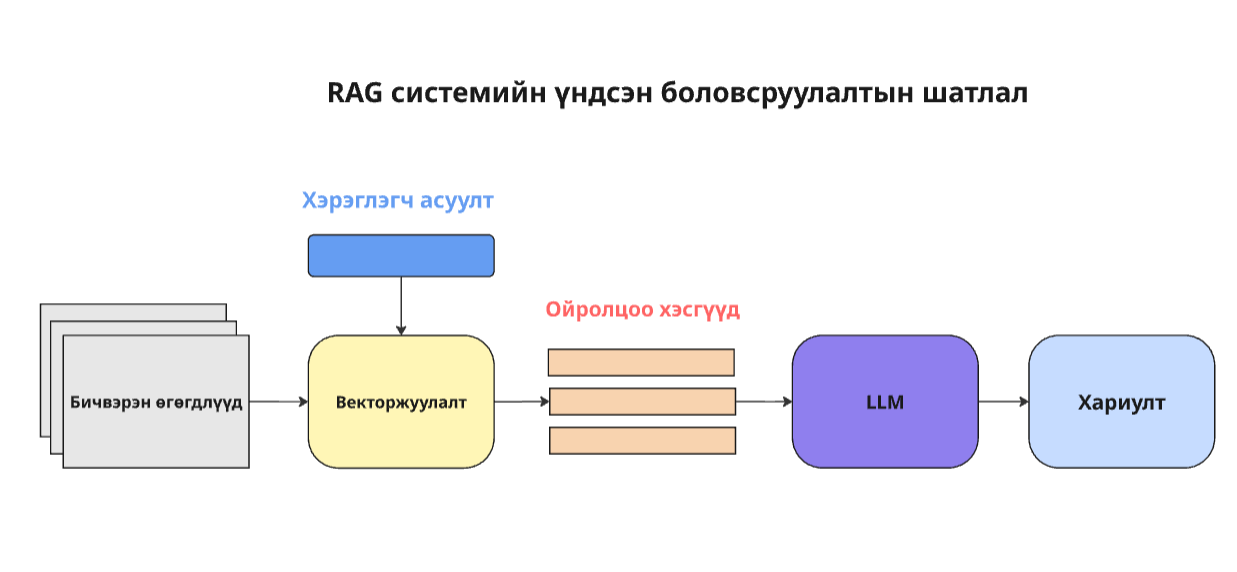
\includegraphics[width=0.8\textwidth]{zurag1.png}
\caption{RAG-ийн үндсэн бүтэц}
\label{fig:rag_structure}
\end{figure}

\subsubsection*{3.1.1 Retriever бүрэлдэхүүн}

Retriever нь RAG-ийн ``хайлт'' хэсгийг хариуцдаг:

\begin{enumerate}
    \item \textbf{Indeksing үе} — Бичвэрүүдийг embedding загвараар тоон вектор болгон FAISS индексэд хадгална.
    \item \textbf{Query боловсруулах үе} — Хэрэглэгчийн асуултыг мөн адил вектор болгон хөрвүүлнэ.
    \item \textbf{Хайх үе} — Хоёр вектор хоорондын косинус зайгаар хамгийн ойрхон утгатай баримтыг олдог.
\end{enumerate}

\subsubsection*{3.1.2 Generator (LLM) бүрэлдэхүүн}

Generator нь Retriever (Мэдээлэл хайгч модуль)-ээс олж ирсэн холбогдох мэдээлэл дээр үндэслэн хүнд ойлгомжтой хариулт үүсгэдэг хэлний загвар юм. RAG технологид Generator нь зөвхөн LLM-ийн өмнө сурсан мэдлэгт тулгуурлахгүй, харин Retriever-ээс авчирсан баримт болон лавлах мэдээллийг уншиж боловсруулан хариулт гаргадаг. Иймээс бодит эх сурвалжид тулгуурласан хариулт үүсэх боломж нэмэгдэж, буруу эсвэл зохиомол мэдээлэл (hallucination) үүсэх эрсдэл мэдэгдэхүйц багасдаг.
\subsubsection*{3.1.3 Ажиллах ерөнхий дараалал}

\begin{enumerate}
    \item Баримт бичгүүдийг уншиж, chunk хэлбэрт хуваана
    \item Chunk бүрийг embedding загвараар тоон вектор болгон FAISS-д хадгална
    \item BM25 статистик индекс бүтээнэ
    \item Хэрэглэгч асуулт оруулахад гурван аргаар зэрэг хайна
    \item Хамгийн холбоотой Top-K chunk-ийг LLM-д контекст болгон өгнө
    \item LLM хариулт үүсгэж хэрэглэгчид харуулна
\end{enumerate}

\subsection{Хосолмол хайлтын онол}

Нэг хайлтын аргад найдах нь ерөнхий нөхцөлд хамгийн сайн үр дүн өгдөггүй. Вектор хайлт утгачилсан асуултанд давуу ч яг нэг үгийн хайлтанд дутмаг, харин BM25 нь эсрэг зарчмаар ажилладаг. Иймд энэ систем гурван аргыг хослуулсан \textbf{Hybrid} шийдлийг ашигласан.

\subsubsection*{3.2.1 Вектор хайлт (FAISS)}

FAISS сан нь бичвэрийн утга, агуулгыг 384 хэмжээст тоон вектор болгон хувиргаж, косинусын томьёогоор векторуудын хоорондын зайг тооцоолон хамгийн ойролцоо утгатай баримтыг олдог. FAISS индексийн хоёр горим:

\begin{itemize}
    \item \textbf{IndexFlatIP} — Бүх векторуудыг шууд харьцуулдаг. Chunk $\le$ 5,000 үед тохиромжтой, нарийвчлал өндөр.
    \item \textbf{IndexIVFFlat} — Векторуудыг $\sqrt{n}$ кластерт хуваан хайдаг. Chunk $>$ 5,000 үед хурд эрс нэмэгддэг.
\end{itemize}

\subsubsection*{3.2.2 Статистик хайлт (BM25)}

BM25 нь баримт бүрийг хэрэглэгчийн хайсан үгтэй хэр тохирч байгаагаар оноогоор эрэмбэлдэг:

\[
  \text{BM25}(q,d) = \sum_{t \in q}
    \log\!\left(\frac{N - n_t + 0.5}{n_t + 0.5}+1\right)
    \cdot
    \frac{f_{t,d}\,(k_1+1)}{f_{t,d} + k_1\!\left(1-b+b\,\frac{|d|}{\text{avgdl}}\right)}
\]

Энд $N$ нийт баримтын тоо, $n_t$ тухайн үг агуулсан баримтын тоо, $k_1=1.5$, $b=0.75$.

\subsubsection*{3.2.3 Шууд тэмдэгтийн хайлт (Keyword Matching)}

Текст доторх үг, тэмдэгтүүдийг яг ижил дарааллаар нь харьцуулдаг энгийн боловч үр дүнтэй арга. Нэр, код, дугаар, тусгай нэр томьёо зэрэг яг ижил хэлбэрээр бичигдсэн мэдээллийг олоход тохиромжтой.

\subsubsection*{3.2.4 Гурван аргын эцсийн нэгтгэл}

\[
  \text{Score}_{\text{total}} =
            w_v \times V_{\text{score}} +
            w_b \times B_{\text{score}} +
            w_k \times K_{\text{score}}
\]

Энд $V$ — FAISS вектор оноо, $B$ — BM25 оноо, $K$ — түлхүүр үгийн оноо.

 \texttt{enhanced\_search\_pipeline()} функц нь асуултын агуулгыг 
шинжилж, түүнд тохирох жингүүд ($w_v, w_b, w_k$)-ийг 
\texttt{WEIGHT\_PROFILES}-оос сонгон ашигладаг. Эдгээр жин нь 
векторын төстэй байдал, текстийн давтамж дээр суурилсан хайлт 
(BM25), мөн түлхүүр үг таарах зэрэг хүчин зүйлүүдийн 
нөлөөллийг тодорхойлдог.
      
Асуултуудыг агуулгын шинжээр нь дөрвөн төрөлд ангилдаг. 
Үүнд: баримтад суурилсан асуулт, утга агуулгад төвлөрсөн асуулт, 
яг ижил үг хэллэгийг хайх асуулт, мөн эдгээрийг хослуулсан 
ерөнхий асуулт. Төрлөөс нь хамааран хайлтын жинг өөрөөр 
тооцоолдог.

Хэрэв хэлний загвар ашиглах боломжгүй тохиолдолд 
нөөц (fallback) хайлтын горим ажиллана. Энэ үед 
\texttt{store.search()} функц нь векторын төстэй байдал ($V$) 
болон BM25 оноо ($B$)-г $0.45 \times V + 0.40 \times B$ 
харьцаагаар нэгтгэж, дээр нь түлхүүр үг таарсан эсэхээс 
хамаарсан нэмэлт оноо нэмж эцсийн үр дүнг гаргадаг.
\subsection{Embedding (вектор дүрслэл) онол}

\subsubsection*{3.3.1 Word Embedding-ийн хөгжил}\label{sec:tfidf-explained}

Бичвэрийг тоон дүрслэлд хөрвүүлэх арга нь мэдээллийн хайлтын технологийн гол суурь болдог. Энэ салбар нь дараах үе шатаар хөгжсөн:

\begin{itemize}
    \item \textbf{TF-IDF (1972)} --- Баримт дахь үгийн давтамж болон нийт корпусд хэр ховор тохиолдохыг хосолсон анхны статистик арга. Утгачилсан ойролцоо байдлыг тооцоолж чаддаггүй.
    \item \textbf{Word2Vec (2013)} --- Google-ийн Mikolov нарын боловсруулсан нейрон сүлжээнд суурилсан арга. ``King -- Man + Woman = Queen'' хэлбэрийн аналоги харилцааг вектор хэлбэрт илэрхийлэх боломжтой болсон~[15].
    \item \textbf{BERT (2018)} --- Google-ийн Transformer архитектурт суурилсан хоёр чиглэлт хэлний загвар. Үгийн утгыг контекстэд тулгуурлан тодорхойлдог тул нэг үг өөр өөр утгатай тохиолдолд зөв ялгадаг~[16].
    \item \textbf{Sentence-BERT (2019)} --- Siamese нейрон сүлжээний тусламжтайгаар бичвэрийн бүхэл өгүүлбэрийн утгыг нэг вектор болгон дүрслэх загвар. Семантик хайлтад хамгийн тохиромжтой~[4].
\end{itemize}

\subsubsection*{3.3.2 Косинусын ижил төстэй байдал}

Вектор хайлтад хоёр бичвэрийн ойролцоо байдлыг дараах томьёогоор хэмждэг:

\[
  \cos(\theta) = \frac{\mathbf{A} \cdot \mathbf{B}}{\|\mathbf{A}\| \|\mathbf{B}\|}
  = \frac{\sum_{i=1}^{n} A_i B_i}{\sqrt{\sum_{i=1}^{n} A_i^2} \cdot \sqrt{\sum_{i=1}^{n} B_i^2}}
\]

Утга нь $[-1, 1]$ мужид байдаг бөгөөд 1-д ойртох тусам хоёр вектор илүү ижил утгатай гэсэн үг. Энэхүү системд FAISS-ийн \texttt{METRIC\_INNER\_PRODUCT} хэмжүүрийг хэрэглэсэн бөгөөд векторуудыг урьдчилан нормчилсон тохиолдолд энэ нь косинус ижил төстэй байдлтай тэнцүү болдог.

\subsubsection*{3.3.3 Multilingual Embedding загвар}

Монгол хэлийг дэмжихийн тулд олон хэлний загварыг сонгосон. \texttt{paraphrase-multilingual-MiniLM-L12-v2} загвар нь 50 гаруй хэлний өгөгдлөөр сургагдсан бөгөөд хэл хоорондын семантик ижил байдлыг ижил вектор орчинд дүрслэдэг онцлогтой. multilingual-e5-small нь Wang нарын E5 аргачлалд суурилсан бөгөөд текстийг вектор хэлбэрт хувиргахдаа “query:” болон “passage:” гэсэн тусгай угтварыг ашигладаг. Энэ бүтэц нь хэрэглэгчийн асуулт болон баримт бичгийн агуулгыг нэг ижил утгын орон зайд дүрслэх боломжийг олгож, улмаар зөвхөн үгийн давхцлаас хамаарахгүйгээр утгын хувьд ижил төстэй мэдээллийг илрүүлэх нөхцөлийг бүрдүүлдэг. Иймд энэхүү загвар нь монгол хэл дээрх асуултыг англи хэл дээрх баримт мэдээлэлтэй утгын түвшинд харьцуулж, олон хэл дамнасан хайлтын үр дүнг сайжруулах давуу талтай юм.

\subsection{Transformer архитектур ба Attention механизм}

\subsubsection*{3.4.1 Attention механизмын үндэс}

Transformer архитектур нь орчин үеийн ихэнх том хэлний загваруудын (LLM) үндсэн суурь болдог. Энэхүү архитектурын гол ойлголт болох self-attention механизм нь өгүүлбэр доторх үг бүрийг бусад бүх үгтэй нь нэгэн зэрэг харьцуулж, аль үг ямар үгтэй илүү утгын холбоотой болохыг тодорхойлдог арга юм.

Self-attention-ийг дараах байдлаар ойлгож болно: өгүүлбэрийн үг бүр өөрийгөө “асуулт (Query)”, бусад үгсийг “түлхүүр (Key)” болон “утга (Value)” хэлбэрээр төлөөлөн авч үздэг. Ингэснээр тухайн үг нь өөрт хамгийн их хамааралтай бусад үгсийг олж, тэдгээрт илүү их анхаарал хандуулдаг.
\[
  \text{Attention}(Q, K, V) = \text{softmax}\!\left(\frac{QK^T}{\sqrt{d_k}}\right)V
\]

Энд $Q$ (Query), $K$ (Key), $V$ (Value) матриц нь оролтын векторуудаас тооцоологдох бөгөөд $d_k$ нь Key вектор хэмжээ юм.

Математикийн хувьд энэ үйл явц нь үг хоорондын хамаарлыг тооцоолж жинлэх хэлбэрээр илэрхийлэгдэнэ. Өөрөөр хэлбэл үг бүр бусад үгтэйгээ хэр зэрэг холбоотойг оноогоор үнэлж, тэр оноог нормчлон (softmax) магадлалын жин болгодог. Дараа нь эдгээр жинг ашиглан тухайн өгүүлбэрийн мэдээллийг хамгийн чухал хэсгүүдэд төвлөрүүлж нэгтгэдэг. Ингэснээр модель өгүүлбэрийн утгыг зөвхөн дараалалд тулгуурлахгүйгээр, бүх үгсийн хоорондын уялдаа холбоонд үндэслэн илүү нарийвчлалтай ойлгох боломжтой болдог. 
\subsubsection*{3.4.2 LLM-ийн бичвэр үүсгэх чадвар}

Том хэлний загварууд нь их хэмжээний бичвэр дээр сургагдсанаар хүний хэлийг ойлгож, хариулт үүсгэх чадвартай болдог. Гэхдээ эдгээр загварт хоёр гол сул тал байдаг:

\begin{itemize}
    \item \textbf{Knowledge cutoff} --- Сургалтын өгөгдлийн хугацааны хязгаараас шинэ мэдээллийг мэдэхгүй.
    \item \textbf{Hallucination} --- Мэдэхгүй зүйлд буруу, гэхдээ итгэлтэй харагдах хариулт үүсгэх хандлага.
\end{itemize}

RAG технологи нь яг эдгээр сул талыг нөхдөгөөрөө онцлог юм: загварын сургагдсан мэдлэг төдийгүй шинэ баримт бичгийн агуулгыг ашигладаг.

\subsection{ONNX ба загварын оновчлолын онол}

\subsubsection*{3.5.1 ONNX стандарт}

ONNX нь нейрон сүлжээний загваруудыг хэрэглэгдэхүүнээс үл хамааран нэгэн стандарт форматад хөрвүүлэхэд зориулагдсан нээлттэй формат юм. Энэхүү стандартын тусламжтайгаар PyTorch, TensorFlow, Keras зэрэг өөр өөр framework дээр хөгжүүлсэн загваруудыг нэгтгэн ONNX формат руу хөрвүүлж, улмаар өөр орчинд дахин хөгжүүлэлт хийх шаардлагагүйгээр шууд ашиглах боломжтой болдог. Ингэснээр загварын хоорондын шилжилт болон тооцооллын явцыг хялбарчилж, хэрэгжүүлж буй орчноос хамаарах хязгаарлалтыг бууруулдаг.
\subsubsection*{3.5.2 INT8 Quantization}

Quantization нь загварын жинг бага нарийвчлалтай тоон хэлбэрт шилжүүлж хэмжээ болон хурдыг сайжруулах арга юм:

\begin{itemize}
    \item \textbf{FP32} --- Стандарт 32-bit float. Нарийвчлал өндөр, хурд удаан.
    \item \textbf{FP16} --- 16-bit float. GPU-д тохиромжтой, FP32-аас $\sim$2 дахин хурдан.
    \item \textbf{INT8} --- 8-bit integer. CPU-д хамгийн тохиромжтой, FP32-аас $\sim$4 дахин хурдан, нарийвчлалын алдагдал 1\% хүрэхгүй.
\end{itemize}

ONNX Runtime-д ашиглагддаг квантчилал нь нейрон сүлжээний загварын тоон утгуудын нарийвчлалыг багасгаж, загварын хэмжээг багасгах болон ажиллах хурдыг нэмэгдүүлэх арга юм. Жишээлбэл, ихэнх загварууд жингүүдээ 32-битийн бутархай тоогоор (FP32) хадгалдаг бол квантчиллын үед эдгээрийг 8-битийн бүхэл тоо (INT8) болгон хөрвүүлдэг. Ингэснээр санах ойд эзлэх хэмжээ багасч, тооцоолол илүү хурдан гүйцэтгэгдэх боломж бүрддэг.
\subsubsection*{3.5.3 Intel OpenVINO хурдасгал}

Intel OpenVINO нь Intel процессорын боломжуудыг ашиглан нейрон сүлжээний загварын ажиллах хурдыг нэмэгдүүлэх зориулалттай хэрэгсэл юм. Энэ нь процессорт байдаг тусгай зааврууд (жишээлбэл, AVX-512, AMX)-ыг ашигласнаар загварын тооцооллыг илүү хурдан гүйцэтгэх боломжийг олгодог.

ONNX Runtime-д OpenVINOExecutionProvider-ийг ашигласнаар нэмэлт код бичихгүйгээр загварын гүйцэтгэлийг мэдэгдэхүйц сайжруулах боломжтой. Туршилтын үр дүнгээс харахад CPU дээр боловсруулах хурд 7 chunk/с байсан бол OpenVINO ашигласнаар 63 chunk/с болж, ойролцоогоор 9 дахин хурд нэмэгдсэн байна.
\subsection{Мэдээлэл хайлтын үнэлгээний үзүүлэлтүүд}

\subsubsection*{3.6.1 Precision@K ба Recall@K}

Хайлтын системийн чанарыг үнэлэхэд хэрэглэгддэг үндсэн үзүүлэлтүүд нь нарийвчлал (Precision) болон санамж (Recall) юм. Эдгээр нь систем хэрэглэгчийн асуултад хэр зөв болон хэр бүрэн хариулж байгааг хэмждэг.
\[
  \text{Precision@K} = \frac{\text{Хамааралтай олдсон баримт}}{K}
\]
Precision@K (нарийвчлал) нь хайлтын системээс буцаасан эхний K баримтын дотор хэд нь тухайн асуулттай үнэхээр хамааралтай байгааг илэрхийлнэ. Өөрөөр хэлбэл, системийн гаргасан үр дүнгийн зөв байдлын түвшинг хэмждэг үзүүлэлт юм. Жишээлбэл, K=5 үед буцаасан 5 үр дүнгээс 4 нь зөв байвал Precision@5 = 0.8 болно.
\[
  \text{Recall@K} = \frac{\text{Хамааралтай олдсон баримт}}{\text{Нийт хамааралтай баримт}}
\]

Энд $K$ нь хайлтаас буцаасан баримтын тоо. Одоогийн систем жижиг учир нь Top-K параметрийг 1--10 хооронд тохируулах ба утгыг 5 тохиромжтой гэж үзсэн.  

\subsubsection*{3.6.2 Confidence Score}

Энэ системд confidence score-ийг \texttt{calculate\_confidence\_score()} функцээр
суурь retrieval оноон дээр нэмэлт шалгууруудын жинг нэмж тооцоолдог.
Аргазүйн хэсэгт уг тооцооллын хүснэгтэн задаргааг
Хүснэгт 6-д нэгтгэн үзүүлэв.

\subsection{Ижил төрлийн судалгааны ажлуудын харьцуулалт}

\begin{table}[H]
\centering
\caption{Ижил төрлийн системүүдийн харьцуулалт}
\label{tab:comparison}
\small
\begin{tabularx}{\textwidth}{|l|c|c|c|c|X|}
\hline
\textbf{Систем} & \textbf{Офлайн} & \textbf{Hybrid} & \textbf{Формат} & \textbf{Монгол} & \textbf{Онцлог} \\
\hline
Lewis et al.\ RAG & Үгүй & Үгүй & Вики & Үгүй & Анхны RAG судалгаа \\
\hline
LangChain RAG & Үгүй & Зарим & PDF,TXT & Үгүй & API шаарддаг \\
\hline
PrivateGPT & Тийм & Үгүй & PDF,TXT & Үгүй & Зөвхөн 2 формат \\
\hline
Haystack & Тийм & Тийм & Олон & Үгүй & Серверт суурилсан \\
\hline
\textbf{RAG (Анар)} & \textbf{Тийм} & \textbf{Тийм} & \textbf{10+} & \textbf{Тийм} & \textbf{ONNX+OpenVINO} \\
\hline
\end{tabularx}
\end{table}

\begin{enumerate}
    \item \textbf{Lewis et al.\ (2020)} — RAG-ийн анхны судалгаа. DPR + BART загвараар Wikipedia-аас хариулт үүсгэсэн~[1]. Гэвч локал файлд хэрэглэх боломжгүй, офлайн горим дэмжихгүй.
    \item \textbf{LangChain RetrievalQA} — OpenAI API шаарддаг, офлайн орчинд нэмэлт тохиргоо хэрэгтэй~[5]. Хамгийн өргөн хэрэглэгддэг боловч өгөгдлийн нууцлалын асуудалтай.
    \item \textbf{PrivateGPT} — Бүрэн локал ажилладаг ч зөвхөн PDF, TXT дэмждэг, Hybrid хайлт хэрэгжүүлээгүй~[12]. ONNX оновчлол байхгүй тул CPU дээр удаан.
    \item \textbf{Haystack (deepset)} — Серверт суурилсан архитектур тул хэрэглэгчийн компьютерт хүнд~[11]. Pipeline тохиргоо нарийн мэдлэг шаарддаг.
    \item \textbf{Benedetti (2024/2025)} — RAGAS framework-ээр RAG системийг үнэлсэн судалгаа~[8]. API-based тул офлайн ашиглах боломжгүй.
\end{enumerate}

Дээрх харьцуулалтаас харахад ихэнх RAG систем нь нэг хайлтын арга, онлайн API, эсвэл цөөн файлын формат дэмждэг. Энэ систем нь \textbf{Hybrid хайлт (3 арга)}, \textbf{бүрэн сүлжээгүй орчинд}, \textbf{10 файлын формат унших}, \textbf{ONNX оновчлол буюу бага тооцоолол} хослуулсанаараа ялгаатай.

% ── §4 Судалгааны арга зүй ───────────────────────────────────
\newpage
\section{Судалгааны арга зүй}

Энэхүү судалгаа нь хэрэглээний чиглэлийн судалгаа бөгөөд хүмүүсийн хувийн болон компанийн файл, бичиг баримттай харьцах, хайх хугацааг багасган илүү үр дүнтэй ажиллахад чиглэсэн. Чанарын судалгаа ашиглан ямар хиймэл оюун ухааны модел илүү хариулт гаргаж байгааг үнэлсэн.

% ── 4.1 Системийн архитектур ─────────────────────────────────
\subsection{Системийн ерөнхий архитектур}

Систем нь гурван гол давхаргаас бүрдэнэ: оролтын давхарга (файл унших, chunk болгох), индексийн давхарга (FAISS + BM25 + кэш), хариултын давхарга (Hybrid хайлт + LLM + UI). Дараах диаграмм нь системийн өгөгдлийн урсгалыг харуулна.

\begin{figure}[H]
\centering
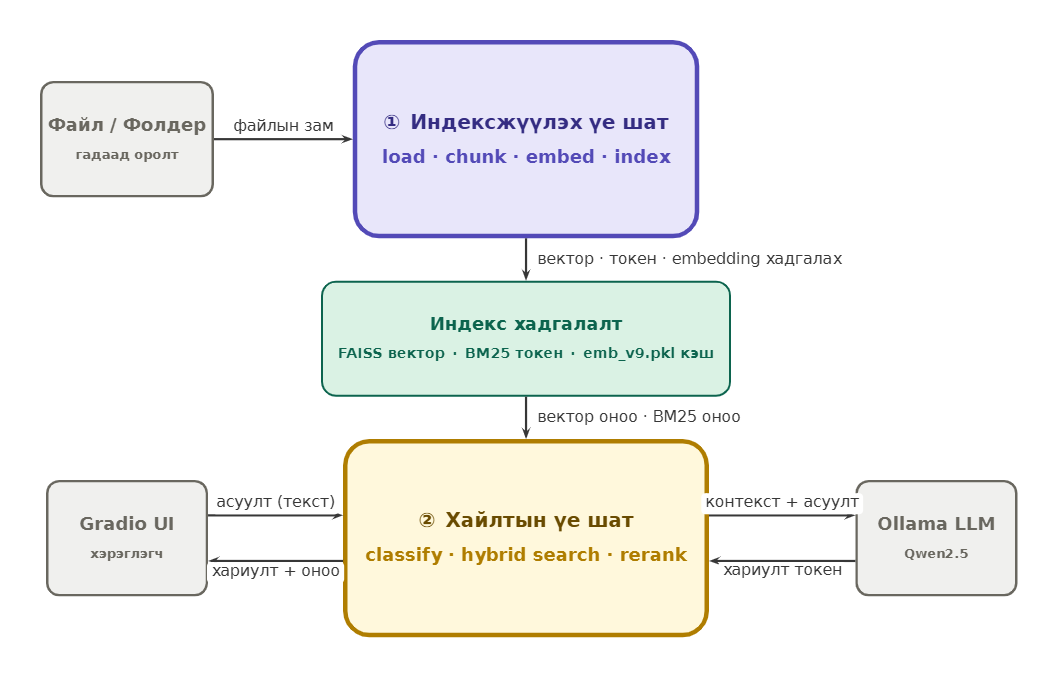
\includegraphics[width=0.8\linewidth,height=0.6\textheight,keepaspectratio]{Зураг2.png}
\caption[Системийн өгөгдлийн урсгал (индексжүүлэлт ба хайлт)]{RAG системийн өгөгдлийн урсгалын диаграмм (DFD): индексжүүлэх үе (файл унших, chunking, embedding, FAISS/BM25) ба хайлтын үе (query боловсруулах, fusion, confidence/rerank, LLM, UI)}
\label{fig:dataflow}
\end{figure}

Зураг~\ref{fig:dataflow}-т үзүүлсэн урсгал нь \texttt{App.py}-ийн бодит хэрэгжилттэй нийцнэ. Индексжүүлэх үед \texttt{load\_documents()} нь файлыг ачаалахаас өмнө хэмжээг (50MB босго) шалгаж, дэмжигдэх өргөтгөлүүдийг шүүдэг. Дараа нь \texttt{chunk\_text()} нь \texttt{CHUNK\_SIZE=600}, \texttt{CHUNK\_OVERLAP=80} тохиргоогоор хэсэгчлэж, \texttt{EmbeddingCache} (\texttt{emb\_v9.pkl})-аар MD5 кэш ашиглан давтагдсан embedding-ийг дахин тооцоолохоос сэргийлнэ. Embedding үүсгэхдээ боломжтой үед ONNX/OpenVINO ашиглаж, боломжгүй үед \texttt{SentenceTransformer} fallback-аар ажиллан, эцэст нь chunk-ийн тооноос хамааран FAISS \texttt{IndexFlatIP} эсвэл \texttt{IndexIVFFlat} болон BM25 индексүүдийг зэрэг хадгалдаг.

Кодын хэрэгжилтийн хариуцлагын түвшинд энэхүү урсгалыг таван модульд товчлон харж болно: M1 (оролт, файл уншилт, шүүлт), M2 (chunk, embedding, индекс), M3 (hybrid retrieval ба confidence), M4 (LLM хариулт үүсгэх), M5 (UI callback ба индексийн lifecycle). Энэ задаргаа нь Зураг~\ref{fig:dataflow}-ийн индексжүүлэх ба хайлтын хоёр үе шаттай логиктой нийцдэг.

% ── 4.2 Ажиллах дараалал ─────────────────────────────────────
\subsection{Системийн ажиллах дараалал}

Систем нь хоёр үндсэн үе шатаар ажилладаг: \textbf{(1) Индексжүүлэх үе} — фолдерын файлуудыг уншиж, chunk болгон (хувааж), embedding + FAISS/BM25 индекс үүсгэж хадгална. \textbf{(2) Хайлтын үе} — хэрэглэгч асуулт оруулахад холимог хайлт хийж, Top-K chunk (хамгийн ойр гэж үзсэн хуваалт)-ийг LLM-д дамжуулан хариулт үүсгэнэ.

\begin{figure}[H]
\centering
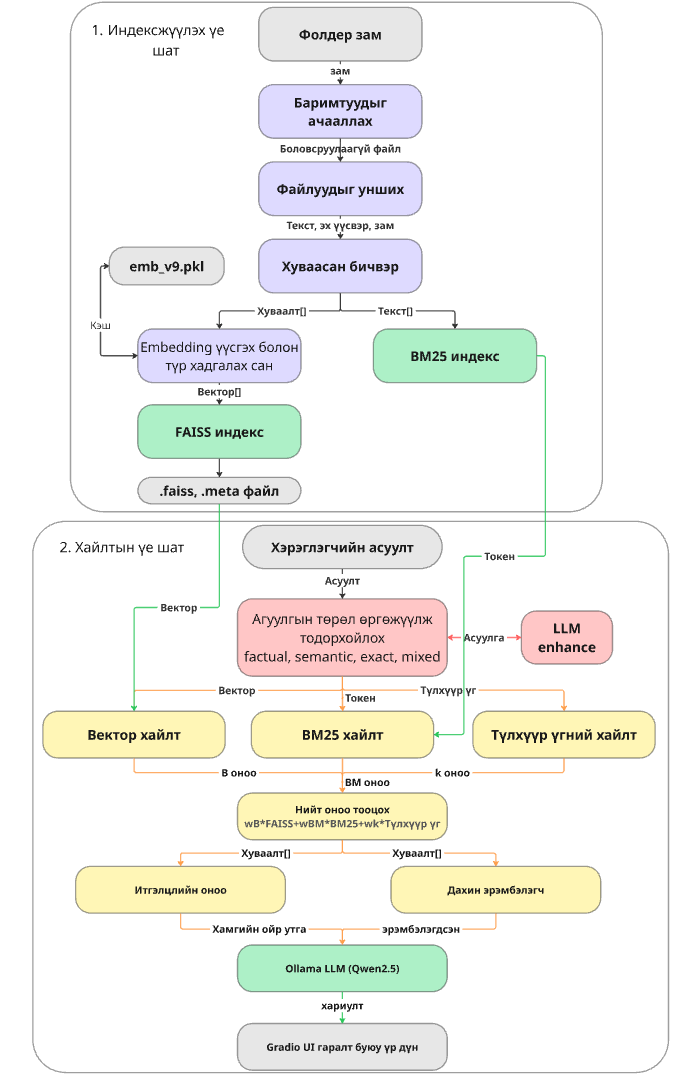
\includegraphics[width=0.8\textwidth]{Зураг3.png}
\caption{Системийн ажиллах дарааллын ерөнхий зураглал}
\label{fig:workflow}
\end{figure}

\noindent Зураг~\ref{fig:workflow}-ийн дагуу ажиллах дарааллыг товчлон үзүүлбэл:
\begin{enumerate}
            \item \textbf{Индексжүүлэх үе:} \texttt{load\_documents()} $\rightarrow$ \texttt{chunk\_text()} $\rightarrow$ \texttt{BM25Index.build(all\_texts)} $\rightarrow$ embedding тооцоолол $\rightarrow$ FAISS индекс $\rightarrow$ \texttt{save()}.
            \item \textbf{Хайлтын үе:} query ангилал + expansion $\rightarrow$ vector/BM25/keyword candidate $\rightarrow$ score fusion $\rightarrow$ (нөхцөлтэй) reranker $\rightarrow$ Top-K context $\rightarrow$ LLM streaming хариулт $\rightarrow$ UI гаралт.
\end{enumerate}

Системийн боловсруулалтын урсгал суурь түвшинд индексжүүлэх үеэс эхэлдэг: энэ алхамыг нэг удаа гүйцэтгэх бөгөөд embedding кэш ашигласнаар зөвхөн өөрчлөгдсөн файлуудыг дахин боловсруулж, тооцооллын зардлыг бууруулна. Үүний дараа хайлтын шатанд асуулгыг \texttt{classify\_query\_type()} болон \texttt{expand\_query()} функцээр шинжилж, \textit{factual} (баримт), \textit{semantic} (утгын), \textit{exact} (шууд таарах), \textit{mixed} (холимог) гэсэн дөрвөн горимын аль жинлэлтийг хэрэглэхийг нөхцөлд тулгуурлан \texttt{WEIGHT\_PROFILES}-оос сонгодог (дэлгэрэнгүйг §4.9.1-д үзнэ үү).

Илүү ахисан түвшинд Ollama загвар сонгогдсон үед \texttt{\_ollama\_ping()} функцээр Ollama LLM ажиллаж байгаа эсэхийг эхэлж шалгана; шалгалт амжилттай бол \texttt{combined\_llm\_enhance()} нь анхны query-г rewritten query болон keywords болгон өргөтгөж, BM25/FAISS-аар нэмэлт candidate таталтын чанар ба хамрах хүрээг сайжруулахад ашиглагдана. Харин \texttt{hyde\_generate()} болон \texttt{self\_reflect\_search()} нь кодод буй нэмэлт helper боломжууд бөгөөд үндсэн \texttt{answer\_stream()} урсгалд заавал ажиллах алхам биш юм. Мөн confidence score нь \texttt{CONFIDENCE\_THRESHOLD=0.65} босготойгоор үр дүнг тайлбарлах дохио хэлбэрээр UI-д харуулагддаг.

% ── 4.3 Файл уншигч ──────────────────────────────────────────
\subsection{Файл уншигч модуль}

Файл уншигч модуль нь \texttt{\_read\_one()} функцаар хэрэгждэг бөгөөд уншилтын урсгалын төв цэг болдог. Энэхүү функц нь хоёр үндсэн үүрэгтэй: файлын төрөлд тохирох уншигчийг автоматаар сонгох, мөн уншилтын үеийн алдааг тогтвортой байдлаар боловсруулах. Уншилт эхлэхээс өмнө урьдчилсан шалгалт хийж, файлын хэмжээг 50MB босготой харьцуулан хэт том файлыг алгасахын зэрэгцээ хоосон файлыг уншилтанд оруулахгүй.

\subsubsection*{4.3.1 Дэмжигдэх форматууд}

Модуль дэмждэг файлын төрлүүд болон тэдгээрт ашиглагдах санг Хүснэгт~\ref{tab:file_extensions}-д нэгтгэн үзүүлэв.

\begin{table}[H]
\centering
\caption{Дэмжигдэх файлын төрлүүд ба уншигч}
\label{tab:file_extensions}
\begin{tabular}{|c|l|l|}
\hline
\textbf{Өргөтгөл} & \textbf{Тайлбар} & \textbf{Ашигласан сан} \\
\hline
.pdf  & Баримт бичиг   & PyMuPDF / pdfplumber / pypdf (4 шатлал) \\
.docx & Word баримт    & python-docx \\
.txt, .md, .log, .rst & Текст файлууд & Built-in (4 encoding дэмжинэ) \\
.csv, .tsv & Хүснэгт   & pandas \\
.xlsx, .xls & Excel    & pandas (openpyxl) \\
\hline
\end{tabular}
\end{table}

Энэхүү хамрах хүрээ нь баримт бичиг, хүснэгтэн өгөгдөл, энгийн текстийн нийтлэг хэрэглээг бүрэн дэмжих зорилготой бөгөөд дараах дэд хэсгүүдэд тайлбарлах шүүлт, нөөц шилжилтийн механизмуудтай уялдан ажилладаг.

\subsubsection*{4.3.2 Encoding автоматаар илрүүлэх}

Текст файл унших үед \texttt{read\_txt()} функц файл зөв уншигдаж байгаа эсэхийг шалгахын тулд UTF-8, UTF-16, CP1251, Latin-1 гэсэн хэд хэдэн хэлбэрээр дарааллаар туршиж үздэг. Аль хэлбэрээр файл алдаагүй уншигдвал түүнийг ашиглан текстийг авна. Ингэснээр Монгол кирилл агуулгыг CP1251 хэлбэрээр хадгалсан хуучин файлуудыг ч алдаагүй унших боломжтой болдог.
\subsubsection*{4.3.3 PDF-ийн 4 шатлалт нөөц шилжилтийн механизм}

PDF файлаас текст гарган авах нь бүтэц, фонт, кодчиллын ялгаанаас шалтгаалан хамгийн эмзэг үе шат тул \texttt{read\_pdf()} функцийг дараах 4 шатлалт нөөц шилжилтийн механизмаар хэрэгжүүлсэн:

\begin{enumerate}
    \item \textbf{PyMuPDF — Шатлал 1 (хамгийн хурдан):}
      \texttt{fitz.open()} функцаар PDF-ийг нээж, хуудас бүрээс \texttt{get\_text("text")} аргаар текст гаргана.Хэрэв гарсан текст хоосон эсвэл хэт богино байвал \texttt{get\_text("dict")} аргыг ашиглан баримт бичгийн жижиг хэсгүүдийн (span) текстийг тус тусад нь цуглуулж авна. Ингэснээр баримтын доторх үг, өгүүлбэрийн хэсгүүдийг алдалгүй унших боломжтой болдог. Харин цуглуулсан текст 10-аас дээш тэмдэгттэй байвал түүнийг амжилттай уншигдсан гэж үзээд шууд буцаана.

    \item \textbf{pdfplumber — Шатлал 2 (CJK/Японы PDF):}
      Япон, хятад фонттой PDF дээр PyMuPDF хангалттай текст гаргаж чадахгүй тохиолдолд \texttt{ pdfplumber.open()} функцийг ашиглан  \texttt{pg.extract\_text()} аргаар хуудас бүрийг уншина.

    \item \textbf{pypdf — Шатлал 3 (ерөнхий нийцтэй):}
      Эхлээд файлын эхний 4 байтыг \texttt{b"\%PDF"} тэмдэгт мөртэй тохирч байгаа эсэхээр PDF формат мөн эсэхийг тодорхойлно. Нөхцөл хангагдвал \texttt{PdfReader(strict=False)} ашиглан хуудас тус бүрийн текстийг уншина. Хэрэв файл нь scan хийсэн зурган PDF бол ``бичвэр гарахгүй'' гэдгийг командын хэсэгт мэдэгдэнэ.

    \item \textbf{Placeholder — Шатлал 4 (файлыг хэзээ ч чимээгүй алдахгүй):}
      Дээрх гурван шат амжилтгүй болсон тохиолдолд PyMuPDF номын санг ашиглан PDF файлын хуудасны тоог тодорхойлж, \texttt{[Зурган PDF] нэр | N хуудас} хэлбэрийн түр орлуулагч текст үүсгэнэ. Ингэснээр тухайн файл нь индексэд бүртгэгдэж, хайлтын үр дүнд харагдах боломжтой болох ба хэрэглэгчдэд уг файл нь зөвхөн зурган хэлбэрийн PDF гэдгийг мэдээллэнэ.
\end{enumerate}

\subsubsection*{4.3.4 Шүүлтийн механизм}

Файлуудыг уншиж индексжүүлэхээс өмнө систем нь өгөгдлийн чанарыг хангах болон боловсруулалтын гүйцэтгэлийг сайжруулах зорилгоор хэд хэдэн шаталсан шүүлтийг хэрэгжүүлдэг.

\begin{itemize}
    \item \textbf{Директорийн шүүлт} --- Хувилбарын удирдлагын сан, виртуал орчин, кэш болон тестийн директор зэрэг техникийн зориулалттай хавтаснуудыг автоматаар алгасна. Шалгалтыг тухайн файлын байрлаж буй замын бүх дээд директорийг хамруулан гүйцэтгэнэ.
    
    \item \textbf{Файлын төрлийн шүүлт} --- Програмын эх код, хоёртын файл болон медиа төрлийн файлуудыг индексжүүлэх үйл явцаас хасна. Ингэснээр текстэн агуулгатай баримт бичгүүдийг боловсруулахад төвлөрөх боломж бүрддэг.
    
    \item \textbf{Тусгай файлын шүүлт} --- Системийн түр файлууд, template бүтэцтэй файл болон тестийн өгөгдөлд хамаарах файлуудыг автоматаар ялган алгасна.
    
    \item \textbf{Хэмжээ болон агуулгын шүүлт} --- Хэт том хэмжээтэй файлууд, хоосон файл, эсвэл маш бага хэмжээний текст агуулсан файлуудыг индексжүүлэхээс өмнө шүүнэ.
    
    \item \textbf{Параллель боловсруулалт} --- Олон файлыг зэрэг унших боломжтой олон урсгалт боловсруулалтыг ашигласнаар нийт индексжүүлэх үйл явцын хурдыг нэмэгдүүлдэг.
\end{itemize}

% ── 4.4 Chunking ─────────────────────────────────────────────
\subsection{Chunking (хэсэгчлэл)}

\texttt{chunk\_text()} функц нь баримт бичгийн текстийг тогтмол урттай жижиг хэсгүүдэд хуваах үүрэгтэй. Кодын тохиргоонд нэг хэсгийн хэмжээг \texttt{CHUNK\_SIZE = 600}, тэмдэгт гэж, харин дараалсан хоёр хэсгийн хооронд давхцах хэмжээг \texttt{CHUNK\_OVERLAP = 80} тэмдэгт гэж тодорхойлсон. Өөрөөр хэлбэл, шинэ хэсэг үүсэх үед өмнөх хэсгийн сүүлийн 80 тэмдэгт давхар орж ирдэг бөгөөд ингэснээр текстийн утга, өгүүлбэрийн уялдаа алдагдахгүй хадгалагддаг.

\subsubsection*{4.4.1 Хуваах алгоритм}

\begin{enumerate}
      \item Бичвэрийн олон давхар зайг \texttt{re.sub(r"\textbackslash s+", " ", text)} илэрхийллээр нэг зай болгон цэвэрлэнэ.
      \item Бичвэрийн урт хуваалтын хэмжээнд хүрмэгц хуваалтыг эхлүүлнэ.
      \item Хуваах цэгийг хэсгийг тасалдалтын дарааллаар \texttt{". "}, \texttt{".\textbackslash n"}, \texttt{"!\textbackslash n"}, \texttt{"?\textbackslash n"}, \texttt{"\textbackslash n\textbackslash n"}, \texttt{"\textbackslash n"}, \texttt{"; "}, \texttt{", "}, \texttt{" "} гэж шалгана.
      \item Overlap хэсгийг дахин оруулахдаа \texttt{start = end - overlap} томьёог ашиглана.
      \item \texttt{MIN\_CHUNK\_LEN = 10} нөхцөлийн дагуу 10 тэмдэгтээс богино chunk-ийг хасна.
\end{enumerate}

\subsubsection*{4.4.2 Chunk мета өгөгдөл}

Текстийг хэсгүүдэд хуваасны дараа chunk бүртэй холбоотой нэмэлт мэдээллийг мета өгөгдөл хэлбэрээр хадгална. Үүнд дараах мэдээллүүд багтана.
\begin{itemize}
    \item \texttt{text} --- chunk-ийн бичвэрийн агуулга
    \item \texttt{source} --- эх файлын нэр (Unicode NFC normalize хийгдсэн)
    \item \texttt{path} --- файлын бүтэн зам
\end{itemize}

\subsubsection*{4.4.3 Параллель chunking}

\texttt{build\_chunks\_parallel()} функц нь \texttt{ThreadPoolExecutor}-ийг ашиглан олон файлыг зэрэгцүүлэн chunk болгон хуваадаг. Файл бүрийн chunk-уудыг \texttt{file\_chunks}-д \texttt{\{path: [chunks]\}} бүтэцтэйгээр хадгална.
% ── 4.5 Embedding ─────────────────────────────────────────────
\subsection{Embedding ба ONNX оновчлол}

\subsubsection*{4.5.1 EmbedEngine класс}

\texttt{EmbedEngine} класс нь lazy loading зарчмаар ажилладаг. Өөрөөр хэлбэл, embedding үүсгэх \texttt{encode()} функц анх дуудагдах үед л загварыг санах ойд ачаална.

Embedding тооцоолох загварыг систем дараах дарааллаар сонгоно.

\begin{enumerate}
\item Хэрэв CPU горимд ажиллаж байгаа бөгөөд ONNX загвар байрлах хавтас илэрвэл \texttt{ORTModelForFeatureExtraction} ашиглан embedding үүсгэнэ.
\item Хэрэв OpenVINO боломжтой бол Intel процессорын хурдасгалыг ашиглан тооцооллыг хурдан гүйцэтгэнэ.
\item Хэрэв OpenVINO ашиглах боломжгүй бол \texttt{model\_q8.onnx} (INT8 квантчилсан загвар) эсвэл \texttt{model.onnx} (FP32 загвар)-ыг ашиглана.
\item Хэрэв ONNX загвар байхгүй бол \texttt{SentenceTransformer} номын сангийн PyTorch загварыг ашиглан embedding үүсгэнэ.
\item Мөн GPU (CUDA эсвэл MPS) боломжтой бол тооцооллыг автоматаар GPU дээр гүйцэтгэнэ.
\end{enumerate}

Ингэснээр систем нь тухайн төхөөрөмжийн боломжит хамгийн тохиромжтой загвар болон тооцооллын орчныг автоматаар сонгож, текстийг вектор хэлбэрт хөрвүүлэх (embedding үүсгэх) ажиллагааг гүйцэтгэдэг.
\subsubsection*{4.5.2 Загварын сонголт}

\begin{table}[H]
\centering
\caption{Embedding загварууд}
\label{tab:embed_models}
\small
\begin{tabularx}{\textwidth}{|>{\raggedright\arraybackslash}X|>{\raggedright\arraybackslash}X|c|c|c|}
\hline
\textbf{Түлхүүр нэр} & \textbf{HuggingFace загвар} & \textbf{Хэмжээ} & \textbf{Монгол} & \textbf{Урт} \\
\hline
Олон хэлний хурдан горим       & paraphrase-multilingual-MiniLM-L12-v2 & 470MB & Тийм & 384 \\
Олон хэлний өндөр чанарын горим & intfloat/multilingual-e5-small        & 470MB & Тийм & 384 \\
Маш хурдан горим               & paraphrase-MiniLM-L3-v2               & 17MB  & Үгүй & 384 \\
Хурдан горим                   & all-MiniLM-L6-v2                      & 80MB  & Үгүй & 384 \\
\hline
\end{tabularx}
\end{table}

Өгөгдмөлөөр \textbf{Олон хэлний хурдан горим} (\texttt{multilingual-fast}) загварыг ашигладаг. \textbf{Олон хэлний өндөр чанарын горим} (\texttt{multilingual-e5-small}) загварыг сонгох үед \texttt{use\_prefix=True} тохиргоог идэвхжүүлж, асуулгад \texttt{"query: "}, баримтад \texttt{"passage: "} гэсэн угтвар нэмж embedding үүсгэнэ. Ингэснээр загвар тухайн текст асуулга эсвэл баримт болохыг зөв ялгаж ойлгож, асуулга болон холбогдох баримтын утгын хамаарлыг илүү оновчтой тодорхойлсноор хайлтын нарийвчлалыг сайжруулдаг.

\subsubsection*{4.5.3 ONNX INT8 quantization}

ONNX нь нейрон сүлжээний загварыг янз бүрийн програм, тооцооллын орчинд ажиллуулах боломж олгодог загварын стандарт формат юм. Загварыг ONNX формат руу хөрвүүлсний дараа INT8 quantization хийснээр жингүүдийг бага нарийвчлалтай (8 бит) хэлбэрт хувиргаж, загварын хэмжээг багасгана. Үүний үр дүнд загварын хэмжээ ойролцоогоор 50%-иар буурч, CPU дээр гүйцэтгэх тооцооллын хурд 2–3 дахин нэмэгддэг.

Мөн Intel процессорт зориулсан OpenVINO provider ашиглах боломжтой үед ONNX загварыг Intel-ийн тусгай хурдасгал ашиглан ажиллуулдаг тул гүйцэтгэлийн хурд дахин 3–5 дахин нэмэгдэх боломжтой. Quantization хийсний дараа үүссэн ONNX загварыг \texttt{model\_q8.onnx} нэртэй файлаар хадгалдаг.

\subsubsection*{4.5.4 GPU-д тулгуурласан batch хэмжээний оновчлол}

Систем нь embedding тооцоолох үед batch хэмжээ (нэг дор боловсруулах текстийн тоо)-г төхөөрөмжийн санах ойн хэмжээнд үндэслэн автоматаар тохируулдаг.

\texttt{\_gpu\_batch()} функц нь GPU-ийн VRAM хэмжээг шалгаж batch хэмжээг нэмэгдүүлнэ. Жишээлбэл, 16GB ба түүнээс их VRAM-тай бол batch хэмжээг 8 дахин, 8GB үед 4 дахин, 4GB үед 2 дахин нэмэгдүүлнэ. Харин GPU ашиглахгүй, зөвхөн CPU дээр ажиллаж байгаа тохиолдолд batch хэмжээг өөрчлөхгүй.

Мөн системийн RAM хэмжээг харгалзан \texttt{\_opt\_batch()} функц тохиромжтой batch хэмжээг сонгодог. Үүнд 8GB хүртэл RAM-тай үед 8, 16GB үед 16, 32GB үед 32, түүнээс их RAM-тай бол 64 хэмжээтэй batch ашиглана.

Ингэснээр систем нь төхөөрөмжийн нөөцийг үр ашигтай ашиглаж, embedding тооцооллыг илүү хурдан гүйцэтгэх боломжтой болдог.

% ── 4.6 Embedding кэш ─────────────────────────────────────────
\subsection{Embedding кэш систем}

\texttt{EmbeddingCache} анги нь embedding-ийг олон дахин тооцоолохоос сэргийлэх зорилгоор MD5 дээр суурилсан хоёр түвшний кэшийн механизм ашигладаг. Өөрөөр хэлбэл өмнө нь боловсруулсан бичвэрийн embedding-ийг хадгалж, дараагийн удаа шууд ашиглах боломжийг олгодог.

Кэшийн ажиллах зарчим

\begin{enumerate}
\item Текстийн хэсэг (chunk) бүрээс MD5-д суурилсан давтагдашгүй таних утга үүсгэнэ. Энэ нь тухайн текстийг өвөрмөц байдлаар танихад ашиглагдана.
\item Програм эхлэх үед өмнө хадгалсан embedding-үүдийг \texttt{emb\_v9.pkl} файлаас санах ойд ачаална.
\item Encoding буюу кодыг тайлж унших үед кэшийг шалгаж, өмнө нь тооцоологдсон бичвэр байвал embedding-ийг шууд ашиглана. Ингэснээр давхардсан бичвэрийг дахин тооцоолох шаардлагагүй болно.
\item Шинээр үүссэн embedding-үүдийг кэшд нэмээд, үндсэн процессыг саатуулахгүйгээр тусдаа процессын урсгал ашиглан хадгална.
\item Кэш файлыг хадгалахдаа эхлээд .tmp түр файлд бичиж, дараа нь солих зарчмаар хадгалж явна.
\end{enumerate}

Ингэснээр embedding тооцооллыг дахин давтахгүй, системийн хурд болон үр ашигийг сайжруулдаг.
% ── 4.7 FAISS ─────────────────────────────────────────────────
\subsection{FAISS вектор индекс}

\texttt{HybridStore.build()} автоматаар сонгодог. Ингэснээр жижиг өгөгдөл дээр өндөр нарийвчлалтай хайлт хийх, харин том өгөгдөл дээр хурдан хайлт хийх хоёрын тэнцвэрийг хангана.

\begin{itemize}
      \item Chunk $\le$ 5,000 үед \textbf{IndexFlatIP} --- индексийг ашиглана. Энэ нь бүх векторуудыг шууд харьцуулж хайлт хийдэг тул нарийвчлал өндөр боловч том өгөгдөл дээр удаан болно.
      \item Chunk $>$ 5,000 үед \textbf{IndexIVFFlat} --- индексийг ашиглана.индексийг ашиглана. Энэ үед систем эхлээд векторуудыг төстэй байдлаар нь бүлэглэн хэсгүүдэд хуваадаг (өөрөөр хэлбэл ижил төрлийн мэдээллүүдийг нэг ангилалд оруулна). Дараа нь хайлтын үед бүх өгөгдлийг шалгахын оронд зөвхөн тухайн асуулгад хамгийн ойр хэсгүүдийг л шалгаж, илүү хурдан хайлт хийдэг.
\end{itemize}

Индексийг .faiss өргөтгөлтэй файлд хадгална. Энэ файл нь embedding векторуудын хайлтын бүтэц буюу үндсэн индексийг агуулдаг. Харин мета өгөгдөл болох chunk-ийн жагсаалт, ашигласан embedding загварын нэр, хадгалсан огноо зэрэг нэмэлт мэдээллийг .meta өргөтгөлтэй pickle файлд тусад нь хадгална. Ингэснээр хайлтын индекс болон тайлбар мэдээллийг хооронд нь ялгаж, системийг илүү зохион байгуулалттай, удирдахад хялбар болгодог.
% ── 4.8 BM25 ──────────────────────────────────────────────────
\subsection{BM25 статистик индекс}

Түлхүүр үгт суурилсан хайлтыг хэрэгжүүлэхдээ систем нь BM25 алгоритмыг ашигладаг. Энэхүү алгоритм нь баримт бичгүүдийн дундаас хэрэглэгчийн асуулгад хамгийн их хамааралтай хэсгүүдийг түлхүүр үгийн давтамж болон тархалтад үндэслэн эрэмбэлж олдог. Хэрэв уг алгоритмыг хэрэгжүүлэх шаардлагатай програмын сан системд суусан байхгүй тохиолдолд орлуулах механизм (fallback) идэвхжиж, TF-IDF дээр суурилсан хайлтын аргыг ашиглана [TF-IDF тайлбар: §3.3.1, х.~\pageref{sec:tfidf-explained}]. Ингэснээр гадны сан дутуу байсан ч системийн үндсэн хайлтын ажиллагаа тасалдахгүй үргэлжлэх боломж бүрддэг.
\subsubsection*{4.8.1 Токенчлох арга}

\texttt{\_tokenize()} функц нь текстийг хэлний онцлогоос хамааран хэсэглэж, латин болон кирилл үгс, мөн CJK (Хятад, Япон, Солонгос) тэмдэгтүүдийг тус тусад нь ялган боловсруулдаг.

\begin{itemize}
    \item \texttt{re.findall(r'\textbackslash w+', txt)} --- үсэг болон тоон тэмдэгтүүдээс бүрдэх үгсийг ялган авна (латин болон кирилл үгсийг хамарна).
    \item CJK тэмдэгтэд суурилсан текстийн хайлтын дүрэм --- Хятад, Япон, Солонгос хэлний тэмдэгтүүдийг тусад нь ялгана.
\end{itemize}

\subsubsection*{4.8.2 Хайлтын боловсруулалт}

Нэг хайлтын асуулгаас гадна \texttt{\_build\_bm25\_queries()} функц нь асуулгын өргөтгөл (query expansion) болон Ollama загварын мэдлэгээс гаргасан түлхүүр үгсийг ашиглан олон төрлийн BM25 хайлтын чанарыг дэлгэрүүлэх үгнүүд үүсгэдэг. Ингэснээр нэг асуулгыг зөвхөн ганц хэлбэрээр биш, өөр өөр утгын хувилбаруудаар хайж илүү өргөн хүрээтэй үр дүн гаргах боломжтой болдог. Гарсан үр дүнг нэгтгэхдээ нэг индексийн оноо хэд хэдэн удаа давтагдан ирвэл хамгийн өндөр оноог хадгалах зарчмаар ажилладаг бөгөөд энэ нь тухайн баримтын хамгийн сайн тохирох байдлыг илэрхийлнэ. 
% ── 4.9 Hybrid хайлт ──────────────────────────────────────────
\subsection{Холимог хайлтын хэрэгжүүлэлт}

\subsubsection*{4.9.1 Дөрвөн горимын жинлэлт}

Хайлтын асуултын шинж чанарт нийцүүлэн дараах дөрвөн жинлэлтийн профайлыг тодорхойлсон:

\begin{table}[H]
\centering
\caption{Хайлтын горим бүрийн жинлэлт}
\label{tab:weight_profiles}
\begin{tabular}{|l|c|c|c|}
\hline
\textbf{Горим} & \textbf{BM25} & \textbf{Vector} & \textbf{Keyword} \\
\hline
factual  & 0.40 & 0.35 & 0.25 \\
semantic & 0.20 & 0.55 & 0.25 \\
exact    & 0.20 & 0.10 & 0.70 \\
mixed    & 0.30 & 0.40 & 0.30 \\
\hline
\end{tabular}
\end{table}

\begin{figure}[H]
\centering
\begin{tikzpicture}[node distance=3.2cm, auto]
  % Define styles
  \tikzstyle{input} = [rectangle, draw, rounded corners, fill=blue!20, 
                       minimum width=2.5cm, minimum height=0.8cm, thick]
  \tikzstyle{decision} = [diamond, draw, fill=yellow!30, 
                          minimum width=2cm, thick]
  \tikzstyle{process} = [rectangle, draw, rounded corners, fill=blue!15, 
                         minimum width=2.2cm, minimum height=0.8cm, thick]
  \tikzstyle{output} = [rectangle, draw, rounded corners, fill=green!20, 
                        minimum width=2.5cm, minimum height=0.8cm, thick]
  
  % Nodes
  \node [input] (input) {Хэрэглэгчийн асуулт};
  
  \node [decision, below of=input, text width=1.8cm, align=center] (classify) {Асуултын төрлийн сонголт};
  
  % Four classification branches
  \node [process, below of=classify, xshift=-4.7cm] (factual) 
    {Баримтын асуулга};
  \node [process, below of=classify, xshift=-1.5cm] (semantic) 
    {Утгын асуулга};
  \node [process, below of=classify, xshift=1.5cm] (exact) 
    {Яг таарах асуулга};
  \node [process, below of=classify, xshift=4.8cm] (mixed) 
    {Холимог асуулга};
  
  % Weight assignments
  \node [fill=blue!10, rounded corners, text width=3.2cm, 
         below of=factual, yshift=-0.3cm, minimum height=1.2cm] (wf) 
    {BM25: 0.40\\Vector: 0.35\\Keyword: 0.25};
  
  \node [fill=blue!10, rounded corners, text width=3.2cm, 
         below of=semantic, yshift=-0.3cm, minimum height=1.2cm] (ws) 
    {BM25: 0.20\\Vector: 0.55\\Keyword: 0.25};
  
  \node [fill=blue!10, rounded corners, text width=3.2cm, 
         below of=exact, yshift=-0.3cm, minimum height=1.2cm] (we) 
    {BM25: 0.20\\Vector: 0.10\\Keyword: 0.70};
  
  \node [fill=blue!10, rounded corners, text width=3.2cm, 
         below of=mixed, yshift=-0.3cm, minimum height=1.2cm] (wm) 
    {BM25: 0.30\\Vector: 0.40\\Keyword: 0.30};
  
  % Final output
  \node [output, below of=classify, yshift=-7cm] (output) 
    {Жин коэффициентүүд};
  
  % Edges
  \draw [->] (input) -- (classify);
  
  \draw [->] (classify) -- node[above, font=\small] {Баримт} (factual);
  \draw [->] (classify) -- node[above, font=\small] {Утга} (semantic);
  \draw [->] (classify) -- node[above, font=\small] {Яг} (exact);
  \draw [->] (classify) -- node[above, font=\small] {Холимог} (mixed);
  
  \draw [->] (factual) -- (wf);
  \draw [->] (semantic) -- (ws);
  \draw [->] (exact) -- (we);
  \draw [->] (mixed) -- (wm);
  
  \draw [->] (wf) -- (output);
  \draw [->] (ws) -- (output);
  \draw [->] (we) -- (output);
  \draw [->] (wm) -- (output);
\end{tikzpicture}
\caption{Асуултын ангилал ба жин сонголтын урсгал}
\label{fig:query-classification-flow}
\end{figure}

\texttt{classify\_query\_type()} функц нь асуултыг шинжилж горимыг сонгоно: ишлэл болон \textit{яг} гэх үг илэрвэл \textit{exact}; тоон утга, хэдэн/хэзээ/хэн зэрэг асуулгын үг илэрвэл \textit{factual}; яагаад/тайлбарла зэрэг семантик түлхүүр илэрвэл \textit{semantic}; бусад тохиолдлыг \textit{mixed} гэж ангилна.

\subsubsection*{4.9.2 Нэгтгэлийн дараалал}

\texttt{answer\_stream()} функц нь хоёр өөр хайлтын урсгал дээр үндэслэн ажилладаг. Хэрэв Ollama загвар ашиглагдаж байвал сайжруулсан хайлтын урсгал болох \texttt{enhanced\_search\_pipeline()}-ийг ажиллуулна. Харин Ollama ашиглагдаагүй тохиолдолд систем үндсэн хайлтын аргаар \texttt{store.search()} функцийг ашиглан нөөц арга байдлаар үр дүн гаргана. Ингэснээр систем нь загварын тохиргооноос хамаарахгүйгээр үргэлж ажиллах боломжтой болж, тасралтгүй хариу өгөх чадвартай болдог.

\texttt{enhanced\_search\_pipeline()} функцийн үндсэн алхмууд:

\begin{enumerate}
\item Асуултыг эхлээд вектор хэлбэрт хөрвүүлж, FAISS дээр ойролцоо утгатай хуваалтуудыг хайна. Энэ үед хайлтын өргөнийг нэмэгдүүлэхийн тулд \texttt{search\_k = min(max(top\_k*10, 50), n)} тохиргоогоор илүү олон боломжийг авч үздэг.
\item BM25 хайлтыг асуулгын өргөтгөсөн (expanded) хувилбарууд дээр давтан ажиллуулж, илүү өндөр оноотой үр дүнг хадгална.
\item Түлхүүр үгт суурилсан хайлтыг \texttt{\_keyword\_search()} функцаар гүйцэтгэнэ.
\item Хэрэв query-ийн үг файлын нэртэй таарч байвал \texttt{\_ensure\_filename\_candidates()} функцаар тухайн файлын холбогдох chunk-ийг нэмэлтээр хайлтад оруулна.
\item Хувийн шинжтэй асуулт (жишээ нь “my”, “миний”, “надад” гэх үгс орсон) илэрвэл resume, CV, certificate зэрэг мета өгөгдөлтэй chunk-уудад нэмэлтээр +0.45 онооны жин өгнө.
\item Ollama LLM-ээс гарсан нэмэлт түлхүүр үгсийг BM25 хайлтаар дахин боловсруулж, өмнөх үр дүнтэй нэгтгэнэ.
\item Хэрэв \texttt{use\_reranker=True}, \texttt{store.reranker.available=True} нөхцөл биелж, кандидат үр дүн 1-ээс их бөгөөд ASCII хувь 0.7-оос дээш байвал reranker ашиглан үр дүнг дахин эрэмбэлнэ.
\end{enumerate}

\subsubsection*{4.9.3 Файлын нэрэнд тулгуурласан нэмэлт хайлт}

\texttt{\_file\_relevance\_score()} функц нь chunk-ийн эх файлын нэртэй query-ийн үгсийн тохиролтын түвшинг тооцоолдог:
\begin{itemize}
    \item Бүх үг тохирвол $+1.0$ оноо
    \item 67\% тохирвол $+0.75$ оноо
    \item 50\% тохирвол $+0.5$ оноо
    \item Нэг үг тохирвол $+0.3$ оноо
\end{itemize}

\subsubsection*{4.9.4 Confidence Score-ийн хүснэгтэн загвар}

\begin{table}[H]
\centering
\caption[Confidence score тооцооллын бүрэлдэхүүн]{Confidence score тооцооллын бүрэлдэхүүн (\fn{calculate_confidence_score()})}
\label{tab:confidence_breakdown}
\small
\begin{tabularx}{\textwidth}{|X|c|X|}
\hline
\textbf{Бүрэлдэхүүн} & \textbf{Нэмэгдэл} & \textbf{Кодын нөхцөл} \\
\hline
Суурь оноо & 0.00 & \texttt{confidence = score} \\
\hline
Олон аргаар баталгаажсан (2+) & +0.15 & \texttt{match\_methods >= 2} \\
\hline
Олон аргаар баталгаажсан (3+) & +0.10 & \texttt{match\_methods >= 3} \\
\hline
Reranker баталгаа & +0.10 & \texttt{rerank\_score > 0.5} \\
\hline
Файлын релеванс нэмэгдэл & +0.05 & \texttt{\_rel > 0.5} \\
\hline
Асуултын үгийн давхцал & +0.05 & \texttt{word\_hits >= 3} \\
\hline
Дээд хязгаар & -- & \texttt{return min(confidence, 1.0)} \\
\hline
\end{tabularx}
\end{table}

Практикт 0.65-аас дээш оноог \texttt{CONFIDENCE\_THRESHOLD = 0.65} босгоор ``найдвартай'' гэж ангилдаг.

Confidence оноо нь тайлбарлах хоёрдогч дохио бөгөөд candidate-ийн эцсийн эрэмбийг \texttt{enhanced\_search\_pipeline()}-ийн нийлмэл оноо тодорхойлно.

% ── 4.10 Query Expansion ──────────────────────────────────────
\subsection{Асуулт өргөтгөлт (Query Expansion)}

\texttt{expand\_query()} функц нь LRU хэлбэрийн кэш ашиглаж, хайлтын нарийвчлалыг дараах механизмуудаар нэмэгдүүлдэг:

\subsubsection*{4.10.1 Товчилсон үгийн тайлал}

30 гаруй товчилсон үгийг \texttt{\_ABBR} толь бичигт хадгалсан. Жишээ нь:
\begin{itemize}
    \item \texttt{jlpt} $\rightarrow$ \textit{``japanese language proficiency test N1 N2 N3''}
    \item \texttt{ббсб} $\rightarrow$ \textit{``банк бус санхүүгийн байгууллага''}
    \item \texttt{cv} $\rightarrow$ \textit{``curriculum vitae resume''}
    \item \texttt{ai} $\rightarrow$ \textit{``artificial intelligence''}
\end{itemize}

\subsubsection*{4.10.2 Домайн тусгай өргөтгөл}

\texttt{\_DOMAIN\_EXPAND} толь бичигт домайн мэдлэгт суурилсан өргөтгөлүүдийг хадгалсан. Жишээлбэл, \texttt{jlpt} илэрвэл \textit{``N1, N2, N3, N4, N5, japanese language, япон хэл, Nihongo Nouryoku Shiken (JLPT)''} зэрэг нэр томьёог нэмнэ.

\subsubsection*{4.10.3 Хувийн асуулт илрүүлэх}

\texttt{\_PERSONAL\_SIGNALS} бүрдэлд \textit{``my, миний, надад, I''} зэрэг 20 гаруй дохионы үгийг хадгалсан. Эдгээр дохио илэрвэл \textit{``resume, cv, profile, certificate, gpa, намтар, анкет''} зэрэг нэмэлт түлхүүр үгийг автоматаар нэмнэ.

% ── 4.11 LLM хайлт сайжруулалт ──────────────────────────────
\subsection{LLM-д тулгуурласан хайлт сайжруулалт}

\subsubsection*{4.11.1 combined\_llm\_enhance() функц}

Загвар сонгогдсон бөгөөд Ollama холболт боломжтой үед энэ функц нэг дуудалтаар гурван үр дүн гаргана: хайлтанд тохирсон шинэчлэгдсэн асуулт (\texttt{rewritten\_query}), 5--10 хайлтын түлхүүр үг (\texttt{keywords}), хэрэглэгчийн зорилгыг тайлбарласан товч тэмдэглэл (\texttt{intent}). Үр дүнг 32 биттэй дотоод кэшт хадгална.

\subsubsection*{4.11.2 HyDE (Hypothetical Document Embedding)}

HyDE арга нь том хэлний загварыг ашиглан хэрэглэгчийн асуултад таамагласан хариултын текст үүсгэж, уг текстийг embedding болгон хувиргаад вектор хайлтад ашиглах боломжийг олгодог. Ингэснээр асуулт болон баримт бичгийн агуулгын хоорондох утгын зөрүү багасч, илүү хамааралтай баримтуудыг илрүүлэх боломж нэмэгддэг~[18]. Энэхүү боломж нь системд нэмэлт туслах механизм хэлбэрээр хэрэгжсэн.

\subsubsection*{4.11.3 Self-Reflective хайлт}

Self-reflective хайлт нь анхны хайлтын үр дүнг LLM-ээр үнэлүүлж, хангалттай мэдээлэл олдсон эсэхийг шалгах нэмэлт механизм юм. Хэрэв үр дүн хангалтгүй гэж үнэлэгдсэн тохиолдолд асуулгыг дахин боловсруулж, нэмэлт хайлт хийснээр шинэ баримтын хэсгүүдийг үр дүнд нэмж оруулна. Энэхүү арга нь Self-RAG судалгаанд санал болгосон зарчмыг ашиглан хэрэгжсэн~[19].

Эдгээр боломжууд нь системийн туршилт болон сайжруулалтын зорилгоор ашиглагдах нэмэлт урсгалууд бөгөөд үндсэн хариу үүсгэх үйл явцад заавал гүйцэтгэгдэх шаардлагатай алхам биш юм.
% ── 4.12 Reranker ──────────────────────────────────────────────
\subsection{Reranker}

Анхны хайлтын үр дүнг илүү нарийвчлалтай эрэмбэлэхийн тулд систем нь Cross-Encoder загварт суурилсан дахин эрэмбэлэх (reranking) механизмыг ашигладаг. Энэ арга нь асуулт болон олдсон баримтын хэсгийг хамтад нь загварт оруулж хамаарлын оноог тооцоолдог. Харин Bi-Encoder арга нь асуулт ба баримтыг тус тусад нь вектор болгон хувиргаж харьцуулдаг. Иймээс Cross-Encoder нь хоёр текстийн харилцан хамаарлыг илүү нарийвчлалтай үнэлэх боломжтой бөгөөд үр дүнгийн чанарыг сайжруулдаг~[20].
Дуудалтын нөхцөлүүд:
\begin{itemize}
    \item Дахин эрэмбэлэх механизм идэвхжсэн бөгөөд шаардлагатай загвар системд бэлэн байх
    \item Анхны хайлтаар нэгээс олон нэр дэвшигч баримтын хэсэг (candidate chunk) олдсон байх
    \item Хэрэглэгчийн асуулт ихэвчлэн ASCII тэмдэгтээс бүрдсэн, өөрөөр хэлбэл англи хэл дээр байх
\end{itemize}
GPU орчинд боловсруулах үед batch хэмжээг орчны боломжид тохируулан динамикаар сонгодог бөгөөд ихэвчлэн 32 хэмжээтэй batch ашигладаг. Харин CPU орчинд мөн 32 хэмжээтэй batch хэрэглэнэ. Хэрэв санах ойн хүрэлцээгүй (out-of-memory) алдаа илэрвэл систем batch хэмжээг автоматаар 8 хүртэл бууруулж боловсруулалтыг үргэлжлүүлдэг.
% ── 4.13 LLM хариулт үүсгэгч ─────────────────────────────────
\subsection{LLM хариулт үүсгэгч (Ollama)}

\subsubsection*{4.13.1 Ollama платформ}

\texttt{Ollama} нь том хэлний загваруудыг (LLM) локал орчинд ажиллуулах платформ юм. Систем нь \texttt{http://localhost:11434} хаяг дахь REST API-гаар дамжин харилцдаг. REST API нь HTTP протокол ашиглан програмууд хооронд мэдээлэл солилцох интерфэйс бөгөөд үүгээр систем асуулга илгээж, загвараас хариу хүлээн авдаг. Мөн платформын ажиллаж буй эсэхийг шалгах үйлдлийн үр дүнг 30 секундын хугацаанд кэшлэн хадгалснаар давтан шалгалтын зардлыг бууруулдаг.
\subsubsection*{4.13.2 Хоёр аргын дуудлага}

Хариуг үе шаттайгаар (гарах бүрт нь) хүлээн авахдаа систем эхлээд \texttt{Ollama} командын мөрийн интерфэйс (CLI)-ийг ашиглан загварыг ажиллуулахыг оролддог. Хэрэв энэ арга амжилтгүй болбол систем \texttt{/api/generate} REST API ашиглан загварт хүсэлт илгээх нөөц аргыг ашиглана. Ийнхүү хоёр өөр арга ашигласнаар системийн ажиллагааны найдвартай байдлыг нэмэгдүүлдэг. Мөн хариу үүсгэх үйл явц хэт удаашрахаас сэргийлж хугацаа хэтрэх хязгаарыг 600 секундээр тогтоосон.

\subsubsection*{4.13.3 LLM загваруудын харьцуулалт}

\begin{table}[H]
\centering
\caption{LLM загваруудын харьцуулалт}
\label{tab:llm_comparison}
\small
\begin{tabularx}{\textwidth}{|l|c|c|c|c|X|}
\hline
\textbf{Загвар} & \textbf{Параметр} & \textbf{Монгол} & \textbf{tok/с} & \textbf{Чанар} & \textbf{Тайлбар} \\
\hline
flan-t5-base  & 250M & Үгүй   & 18 & **      & Хурдан ч Монгол дэмжихгүй \\
\hline
qwen2:0.5b    & 500M & Тийм   & 14 & ***    & Хөнгөн, Монгол дэмждэг \\
\hline
qwen2:1.5b    & 1.5B & Тийм   & 9  & ****  & Тэнцвэртэй хурд, хариулт сайн \\
\hline
llama3.2:3b   & 3B   & Дундаж & 5  & ****  & Англи сайн, Монгол дутмаг \\
\hline
qwen2:7b      & 7B   & Тийм   & 2  & ***** & Чанар өндөр, RAM ихтэй машинд \\
\hline
llama3:8b     & 8B   & Дундаж & 2  & ****  & Англи асуултанд сайн \\
\hline
\end{tabularx}
\end{table}

Туршилтын үр дүнд \textbf{Qwen2.5} загварыг сонгосон~[22]. Энэ загвар нь Монгол хэлийг дэмждэг, CPU дээр ажиллаж болохуйц хурдтай, мөн 0.5B--7B хүртэлх хувилбаруудтай.

% ── 4.14 Хэрэглэгчийн дэлгэц ─────────────────────────────────
\subsection{Хэрэглэгчийн дэлгэц (Gradio)}

Энэхүү хэсэгт UI-ийн логикийг бодит компонент болон callback-ийн урсгалаар тайлбарлаж, дараах sequence диаграммаар хэрэглэгчээс хариу буцах хүртэлх гол харилцан үйлчлэлийг нэгтгэн үзүүлэв. Энэ нь Зураг~\ref{fig:dataflow}-ийн хайлтын үеийн гаралт UI дээр хэрхэн харагдахыг \texttt{App.py}-ийн хэрэгжилттэй шууд холбож өгдөг.

\begin{figure}[H]
\centering
\begin{tikzpicture}[x=0.86cm,y=0.86cm,font=\small, every node/.style={transform shape}]
      \tikzset{
            seqactor/.style={draw, rounded corners=1.5pt, fill=gray!10, minimum width=2.8cm, minimum height=0.9cm, align=center, font=\small\bfseries},
            seqlifeline/.style={gray!70, dashed, line width=0.7pt},
            seqmsg/.style={-Stealth, line width=0.95pt},
            seqret/.style={-Stealth, dashed, line width=0.9pt},
            seqlabel/.style={font=\scriptsize, fill=white, inner sep=1.3pt, text=black},
            seqphase/.style={gray!65, dashed, line width=0.6pt},
            seqphasetext/.style={anchor=east, font=\footnotesize\bfseries, text=black},
            seqlegendbox/.style={draw, rounded corners=1.5pt, fill=white, line width=0.6pt},
            seqlegendtxt/.style={font=\scriptsize, align=left}
      }

      % X positions (actors)
      \def\xU{0}
      \def\xG{3.9}
      \def\xR{7.8}
      \def\xO{11.7}

      % Vertical extents
      \def\yTop{0}
      \def\yLifetop{-0.8}
      \def\yBottom{-14.8}

      % Actors
      \node[seqactor] (u) at (\xU,\yTop) {Хэрэглэгч};
      \node[seqactor] (g) at (\xG,\yTop) {Gradio UI};
      \node[seqactor] (r) at (\xR,\yTop) {RAG Engine};
      \node[seqactor] (o) at (\xO,\yTop) {Ollama LLM};

      % Lifelines
      \draw[seqlifeline] (\xU,\yLifetop) -- (\xU,\yBottom);
      \draw[seqlifeline] (\xG,\yLifetop) -- (\xG,\yBottom);
      \draw[seqlifeline] (\xR,\yLifetop) -- (\xR,\yBottom);
      \draw[seqlifeline] (\xO,\yLifetop) -- (\xO,\yBottom);

      % Phase guides
      \draw[seqphase] (-1.0,-4.0) -- (13.2,-4.0);
      \draw[seqphase] (-1.0,-8.9) -- (13.2,-8.9);
      \node[seqphasetext] at (-1.2,-2.2) {A. Эхлүүлэх};
      \node[seqphasetext] at (-1.2,-6.4) {B. Индексэлэх};
      \node[seqphasetext] at (-1.2,-11.9) {C. Асуулт $\rightarrow$ Хариулт};

      % --- Phase A: Start-up ---
      \draw[seqmsg] (\xU,-1.2) -- (\xG,-1.2) node[midway,above,seqlabel] {Систем ажиллуулах};
      \draw[seqmsg] (\xG,-2.0) -- (\xR,-2.0) node[midway,above,seqlabel] {Загвар/индекс ачаалах};
      \draw[seqmsg] (\xR,-2.8) -- (\xO,-2.8) node[midway,above,seqlabel] {Модель эхлүүлэх};
      \draw[seqret] (\xO,-3.2) -- (\xR,-3.2) node[midway,below,seqlabel] {Бэлэн};
      \draw[seqret] (\xR,-3.6) -- (\xG,-3.6) node[midway,below,seqlabel] {Индекс/загвар бэлэн};
      \draw[seqret] (\xG,-4.0) -- (\xU,-4.0) node[midway,below,seqlabel] {UI нээгдлээ};

      % --- Phase B: Indexing ---
      \draw[seqmsg] (\xU,-5.0) -- (\xG,-5.0) node[midway,above,seqlabel] {Хавтас сонгох};
      \draw[seqmsg] (\xG,-5.9) -- (\xR,-5.9) node[midway,above,seqlabel] {Индексэлэх хүсэлт};

      % Self processing at RAG
      \draw[seqmsg] (\xR,-6.8) -- (\xR+1.7,-6.8) -- (\xR+1.7,-7.8) -- (\xR,-7.8)
            node[pos=0.52,right,font=\scriptsize,align=left, fill=white, inner sep=1.2pt] {Унших $\rightarrow$ chunk\\$\rightarrow$ embedding $\rightarrow$ хадгалах};

      \draw[seqret] (\xR,-8.3) -- (\xG,-8.3) node[midway,below,seqlabel] {Индекс бэлэн};
      \draw[seqret] (\xG,-8.8) -- (\xU,-8.8) node[midway,below,seqlabel] {Төлөв харуулах};

      % --- Phase C: QA ---
      \draw[seqmsg] (\xU,-9.9) -- (\xG,-9.9) node[midway,above,seqlabel] {Асуулт оруулах};
      \draw[seqmsg] (\xG,-10.8) -- (\xR,-10.8) node[midway,above,seqlabel] {Асуулт илгээх};

      % Retrieval self call
      \draw[seqmsg] (\xR,-11.6) -- (\xR+1.5,-11.6) -- (\xR+1.5,-12.5) -- (\xR,-12.5)
            node[pos=0.52,right,font=\scriptsize, fill=white, inner sep=1.2pt] {Retrieval (top-k)};

      \draw[seqmsg] (\xR,-13.1) -- (\xO,-13.1) node[midway,above,seqlabel] {Prompt + context};
      \draw[seqret] (\xO,-13.6) -- (\xR,-13.6) node[midway,below,seqlabel] {үе шаттай хариу};
      \draw[seqret] (\xR,-14.1) -- (\xG,-14.1) node[midway,below,seqlabel] {Хариу stream};
      \draw[seqret] (\xG,-14.6) -- (\xU,-14.6) node[midway,below,seqlabel] {Хариу харуулах};

\end{tikzpicture}
\caption{RAG системийн ажлын дараалал: эхлүүлэх, индексэлэх, асуулт-хариултын урсгал}
\label{fig:rag-sequence-improved}
\end{figure}

Зураг~\ref{fig:rag-sequence-improved}-д Хэрэглэгч, Gradio UI, RAG Engine, Ollama LLM гэсэн дөрвөн оролцогчийн харилцан ажиллагааг A~Эхлүүлэх, B~Индексэлэх, C~Асуулт$\rightarrow$Хариулт гэсэн гурван үе шатанд системчилсэн байдлаар үзүүлэв. A үе шат нь орчны тохиргоо, үйлчилгээний бэлэн байдлыг хангаж дараагийн боловсруулалтын суурийг бүрдүүлдэг. B үе шатанд баримтын агуулгыг chunk болон embedding хэлбэрт хөрвүүлж индекс үүсгэснээр асуулгад тохирох контекстийг илүү нарийвчлалтай татах боломж нэмэгдэнэ. C үе шатанд retrieval болон генерацын урсгал нэгтгэгдэж, хариуг stream горимоор үе шаттай дамжуулах нь хэрэглэгчийн мэдрэх хүлээлгийн хугацааг бууруулж интерактив байдлыг сайжруулдаг. Мөн аль нэг урсгал түр тасалдсан нөхцөлд орлуулах боловсруулалтын замаар хариу үргэлжлүүлэх боломж хадгалагдсанаар системийн найдвартай ажиллагаа дэмжигддэг.

Gradio 4.0+ хувилбараас \texttt{type="messages"} форматыг дэмждэг бөгөөд \texttt{\_GR\_VERSION} шалгалтаар хуучин хувилбаруудтай нийцтэй байдлыг хадгалдаг. Дэлгэц нь хоёр хэсгээс бүрдэнэ:

\begin{itemize}
      \item \textbf{Асуулт хэсэг} --- градиент дэвсгэртэй гарчиг, чат хэлбэрийн хариулт, хайлтын оноо болон файл бүрийн ranking-ийг харуулдаг. Debug горим идэвхтэй үед оноо болон scoring method-ийн дэлгэрэнгүй мэдээллийг нэмэлтээр гаргана.
      \item \textbf{Файл шалгах хэсэг} --- файлын нэрийн хэсгийг оруулахад тухайн файл индексэд байгаа эсэх, chunk-ийн тоо, тест асуултад авсан оноог харуулдаг. \texttt{diagnose\_file()} функц table detection, vector score, BM25 score, keyword score болон бүх файл дундах rank-ийг нэг дор харуулна.
\end{itemize}

Тохиргооны параметрүүдийг хэрэглэгчийн интерфейс (UI)-ээр дамжуулан шууд өөрчлөх боломжтой. Үүнд хайлтын үр дүнгийн тоог тодорхойлох Top-K параметр (1–10), дахин эрэмбэлэх механизмыг идэвхжүүлэх сонголт, алдааг олох горимын тохиргоо, embedding загварын сонголт
% ── 4.15 Хүндрэлүүд ───────────────────────────────────────────
\subsection{Хөгжүүлэлтийн явцад тулгарсан хүндрэлүүд ба шийдлүүд}

\subsubsection*{4.15.1 Chunking хэмжээ хангалтгүй}

\textbf{Асуудал:} Том файлыг бүхэлд нь нэг embedding болгон боловсруулахад баримтын тодорхой хэсэгт байрласан мэдээллийг олоход хүндрэл үүссэн.

\textbf{Шийдэл:} Chunk-ийн хэмжээг 600 тэмдэгт, overlap-ийг 80 болгон тохируулсан. Үүний үр дүнд нийт chunk тоо буурч, хайлтын нарийвчлал сайжирсан.

\subsubsection*{4.15.2 FAISS dimension mismatch алдаа}

\textbf{Асуудал:} Embedding загварыг өөрчлөх үед ``dimension mismatch'' алдаа тогтмол гарч байсан.

\textbf{Шийдэл:} Индексийг ачаалах үед хэмжээсийг шалгаж, зөрүү илэрвэл хуучин индексийг устган шинээр үүсгэдэг хамгаалалтын логик нэмсэн.

\subsubsection*{4.15.3 PDF уншилтын хүндрэл}

\textbf{Асуудал:} Зурган PDF файлаас текст гарахгүй, улмаар файл чимээгүйгээр алдагдах тохиолдол гарч байсан.

\textbf{Шийдэл:} 4 шатлалт fallback механизм хэрэгжүүлж, Stage 4-т placeholder буцаадаг болгосон. Зурган PDF-д OCR дэмжлэгийг цаашид нэмэх шаардлага хэвээр байна.

\subsubsection*{4.15.4 AI хариулт удаашрах}

\textbf{Асуудал:} Хэт олон chunk дамжуулах үед LLM-ийн хариу удааширч байсан.

\textbf{Шийдэл:} Top-K-ийн өгөгдмөл утгыг 5 болгосон. Мөн streaming горимын ачаар хариулт нэн даруй эхлэх боломжтой болсон.

\subsubsection*{4.15.5 Дахин индексжүүлэх удаашрал}

\textbf{Асуудал:} Системийг дахин ажиллуулах бүрт бүх файлыг дахин embedding хийж байсан.

\textbf{Шийдэл:} MD5 hash-д суурилсан кэшийн систем нэвтрүүлснээр зөвхөн өөрчлөгдсөн файлуудыг боловсруулдаг болсон. Ингэснээр хугацаа 614 секундээс $\sim$5 секунд болж буурсан.

\subsubsection*{4.15.6 Unicode filename зөрүү}

\textbf{Асуудал:} macOS болон Windows орчин дахь Unicode NFC/NFD хэлбэрийн зөрүүнээс шалтгаалан Монгол нэртэй файлуудыг олохгүй байсан.

\textbf{Шийдэл:} Бүх файлын нэрийг \fn{_normalize_filename()} дотор \fn{unicodedata.normalize("NFC", name)} хэлбэрт жигдрүүлдэг болсон. Мөн chunk-ийн \texttt{source} талбарт бичихийн өмнө адил normalize хийдэг болсон.

\subsubsection*{4.15.7 Хэт олон техникийн файл индексэд орох}

\textbf{Асуудал:} Python виртуал орчин, Git репозитори, node\_modules зэрэг хавтсуудын мянга мянган файл индексэд орсноор хурд болон чанар буурч байсан.

\textbf{Шийдэл:} \texttt{IGNORE\_DIRS} бүрдэлд техникийн директоруудыг өргөтгөж, \fn{_should_skip_file()} функцаар fixture, template зэрэг тестийн файлуудыг шалтгаантайгаар алгасдаг болсон.

% ── §5 Үр дүн, дүгнэлт ───────────────────────────────────────
\newpage
\section{Судалгааны үр дүн, дүгнэлт}

Энэ бүлэгт боловсруулсан системийг туршилтын нөхцөлд ажиллуулж гаргасан тоон үр дүнг танилцуулна. Туршилтыг гүйцэтгэлийн хэмжилт, оновчлолын нөлөө, хайлтын нарийвчлалын харьцуулалт, query expansion болон файлын форматын дэмжлэг гэсэн таван чиглэлээр авч үзэв.

% ── 5.1 ──────────────────────────────────────────────────────
\subsection{Гүйцэтгэлийн хэмжилт}

Системийн гүйцэтгэлийг бодитоор хэмжихийн тулд 35~MB-аас 350~MB хүртэлх гурван өөр хэмжээний баримтын сантай туршилт хийсэн. Туршилтын техник хангамжийн орчин: \textbf{Intel Core i7-11800H} (8 цөм, 16 нийлмэл нэгж), \textbf{7.7~GB RAM}, \textbf{Intel Iris Xe Graphics}, Windows~11, Python~3.11, OpenVINO~2024.0.

\begin{table}[H]
\centering
\caption{Системийн бодит гүйцэтгэлийн хэмжилт (CPU горим, Intel OpenVINO)}
\label{tab:benchmark}
\small
\begin{tabular}{|c|c|c|c|c|c|}
\hline
\textbf{Санын хэмжээ} & \textbf{Chunk тоо} & \textbf{Индексэлт (с)} & \textbf{Хайлт (avg)} & \textbf{AI хариулт} & \textbf{Embed хурд} \\
\hline
$\sim$35~MB  & 4,135  & 65с   & 0.018с & 2.1с & 63 chunk/с \\
\hline
$\sim$90~MB  & 12,500 & 195с  & 0.022с & 2.3с & 63 chunk/с \\
\hline
$\sim$350~MB & 60,862 & 614с  & 0.035с & 2.5с & 63 chunk/с \\
\hline
\end{tabular}
\end{table}

Хүснэгт~\ref{tab:benchmark}-ээс харахад санын хэмжээ 10 дахин өссөн ч хайлтын дундаж хурд 0.018с-ээс 0.035с болж зөвхөн $\sim$2 дахин удааширсан байна. Энэ нь FAISS болон BM25 индексүүдийн хайлтын цогцолбор байдал санын хэмжээнд логарифмын хамааралтайгаар өсдөгтэй холбоотой юм. Embedding хурд 63~chunk/с-д тогтвортой хэвээр байгаа нь OpenVINO-ийн batch боловсруулалтын тогтвортой байдлыг харуулна. AI хариултын хугацаа 2.1--2.5с-ийн хооронд хэлбэлзсэн нь Ollama-ийн локал загварын боловсруулалтын хугацааг тусгана.

% ── 5.2 ──────────────────────────────────────────────────────
\subsection{Индексэлэлтийн задаргаа}

350~MB-ийн баримтын санг индексэлэхэд зарцуулсан нийт 614 секундын хугацааг алхам бүрээр задалж судалсан. Уг шинжилгээ нь цаашдын оновчлолын зорилтыг тодруулахад ач холбогдолтой.

\begin{table}[H]
\centering
\caption{350~MB баримтын санг индексэлэхэд зарцуулсан хугацааны задаргаа}
\label{tab:breakdown}
\begin{tabular}{|l|c|c|}
\hline
\textbf{Алхам} & \textbf{Хугацаа (с)} & \textbf{Эзлэх хувь} \\
\hline
Файл уншилт                           & 50с  & 8\%  \\
\hline
Chunking                               & 5с   & 1\%  \\
\hline
BM25 индекс                            & 8с   & 1\%  \\
\hline
Embedding (ONNX INT8 + OpenVINO, 63/с) & 540с & 88\% \\
\hline
FAISS индекс                           & 5с   & 1\%  \\
\hline
Хадгалалт                              & 6с   & 1\%  \\
\hline
\textbf{Нийт}                          & \textbf{614с} & \textbf{100\%} \\
\hline
\end{tabular}
\end{table}

Хүснэгт~\ref{tab:breakdown}-оос тодорхой харагдаж байгаагаар embedding тооцооллын алхам нийт индексэлэлтийн хугацааны \textbf{88\%}-ийг буюу 540~секундийг эзэлж байна. Энэ нь тухайн алхам нь системийн гүйцэтгэлийн хамгийн чухал саад болж байгааг (bottleneck) илтгэнэ. Харин chunking, BM25 болон FAISS индекс үүсгэлт тус бүр нийт хугацааны 1\%-иас хэтрэхгүй байгаа нь эдгээр алхмуудад оновчлол хийх шаардлага бага гэдгийг харуулна.

Embedding-ийн саадыг нэмэгдүүлэхийн тулд хоёр замыг туршив: нэгдүгээрт, GPU-тай тоног төхөөрөмж дээр ажиллуулахад NVIDIA RTX~3060 дээр 614с-аас $\sim$45с болж $\approx$13.7 дахин хурдасч байна. Хоёрдугаарт, MD5 хэш дээр суурилсан кэшийн механизм ашиглан зөвхөн өөрчлөгдсөн файлуудыг дахин боловсруулдаг болгосноор ердийн ажлын нөхцөлд давтан индексэлэлт $\sim$5~секундэд багтдаг болсон.

% ── 5.3 ──────────────────────────────────────────────────────
\subsection{Оновчлолын үр дүн}

Системийн анхны хувилбараас эхлэн хэд хэдэн инженерчлэлийн оновчлол хэрэгжүүлсэн. Доорх хүснэгтэд оновчлол тус бүрийн өмнөх болон дараах хэмжилтийг харуулав.

\begin{table}[H]
\centering
\caption{Оновчлол тус бүрийн хэмжилтийн харьцуулалт}
\label{tab:optimization}
\begin{tabular}{|l|c|c|}
\hline
\textbf{Оновчлол} & \textbf{Өмнөх утга} & \textbf{Дараах утга} \\
\hline
ONNX INT8 тоон хувирал (quantization)    & 4~chunk/с    & 7~chunk/с    \\
\hline
Intel OpenVINO хурдасгал                 & 7~chunk/с    & 63~chunk/с   \\
\hline
Chunk хэмжээ оновчлол (600/80)           & 90,000~chunk & 60,862~chunk \\
\hline
XLSX/CSV их мөртэй шүүлт                & $\sim$100с/файл & $\sim$1с/файл \\
\hline
Embedding MD5 кэш (дахин индексэлт)     & 614с         & $\sim$5с     \\
\hline
FileTracker өөрчлөлтийн хяналт          & бүгдийг дахин боловсруулна & зөвхөн өөрчлөгдсөн файл \\
\hline
\end{tabular}
\end{table}

Хамгийн мэдэгдэхүйц үр дүн нь ONNX INT8 тоон хувирал болон Intel OpenVINO-г хамтад нь хэрэглэснээр embedding хурд 4~chunk/с-ээс 63~chunk/с болж \textbf{15.75 дахин} нэмэгдсэн явдал юм. Chunk хэмжээг оновчилснаар нийт chunk тоо 90,000-аас 60,862-т хүрч 32\%-иар буурсан нь хайлтын нарийвчлал болон RAM-ын ашиглалтад эерэгээр нөлөөлсөн. XLSX/CSV шүүлтийн оновчлол нь их мөртэй хүснэгтийн файлуудыг боловсруулах хугацааг 100 дахин бууруулсан нь систем практик ашиглалтад тохиромжтой болоход чухал хувь нэмэр оруулсан.

% ── 5.4 ──────────────────────────────────────────────────────
\subsection{Хайлтын нарийвчлалын харьцуулалт}

Hybrid хайлтын давуу талыг тодруулахын тулд нэг аргатай болон хослосон аргуудтай шууд харьцуулсан туршилт хийсэн. Нийт 50 асуулт бэлтгэж, ижил баримтын сангаар туршиж, хэрэглэгчийн үнэлгээгээр (human evaluation) зөв хариулт эсэхийг шийдвэрлэсэн. Үнэлгээний үзүүлэлт болгон Information Retrieval-д өргөн хэрэглэгддэг Precision@5 болон Recall@5 хэмжигдэхүүнүүдийг ашиглав.

\begin{table}[H]
\centering
\caption{Хайлтын аргын нарийвчлалын харьцуулалт (50 асуулт, Top-$k$=5)}
\label{tab:precision_compare}
\begin{tabular}{|l|c|c|c|}
\hline
\textbf{Хайлтын арга} & \textbf{Precision@5} & \textbf{Recall@5} & \textbf{Зөв хариулт \%} \\
\hline
Зөвхөн Keyword              & 0.44 & 0.41 & 48\% \\
\hline
Зөвхөн BM25                 & 0.57 & 0.54 & 60\% \\
\hline
Зөвхөн Vector (FAISS)       & 0.61 & 0.58 & 64\% \\
\hline
Vector + BM25                & 0.72 & 0.69 & 74\% \\
\hline
\textbf{Hybrid (3 арга)}     & \textbf{0.81} & \textbf{0.78} & \textbf{84\%} \\
\hline
Hybrid + Reranker            & 0.86 & 0.80 & 88\% \\
\hline
\end{tabular}
\end{table}

Хүснэгт~\ref{tab:precision_compare}-ийн үр дүнгээс хэд хэдэн чухал дүгнэлт гаргаж болно. Нэгдүгээрт, зөвхөн нэг арга ашиглах үед хамгийн сайн гүйцэтгэл нь Vector (FAISS) аргаас 64\%-ийн зөв хариулт гарч байгаа нь бусад аргаас давуу ч гэсэн дангаараа хангалтгүй байна. Хоёрдугаарт, Vector болон BM25-ийг хослуулахад гүйцэтгэл 74\%-д хүрч нэмэлт аргын ашигтай нөлөө тодорхой харагдана. Гуравдугаарт, гурван аргыг нэгэн зэрэг ашигласан Hybrid хайлт \textbf{84\%}-ийн зөв хариулт өгч, дан Vector аргаас \textbf{+20 нэгж хувиар} давж байна. Reranker нэмснээр Precision@5 0.86 болж нэмэгдсэн боловч Монгол хэлний асуултад тусламж бага байсан нь ms-marco загвар нь Монгол хэлний утгын давхцалд хязгаарлагдмал гэдгийг харуулж байна.

% ── 5.5 ──────────────────────────────────────────────────────
\subsection{Query Expansion-ийн үр нөлөө}

Асуулт өргөтгөлтийн (Query Expansion) нөлөөг тодруулахын тулд ижил асуулт дээр өргөтгөлтэй болон өргөтгөлгүй горимыг харьцуулж, хайлтын үр дүнд олдох хамааралтай chunk-ийн тоог тоолов.

Жишээ нь ``JLPT'' гэсэн товчилсон асуулт өргөтгөлгүйгээр хайхад дан \texttt{jlpt} тэмдэгт агуулсан chunk~3 л олдож байсан бол \texttt{expand\_query()} функцийн дараа ``japanese language proficiency'', ``N1'', ``N2'', ``N3'' зэрэг холбогдох нэр томьёог агуулсан chunk-ийг мөн хамруулан нийт~11 болж нэмэгдсэн. Ингэснээр хамааралтай баримтын тоо дунджаар \textbf{2.3 дахин} нэмэгдэж байна.

\begin{table}[H]
\centering
\caption{Query Expansion өргөтгөлийн өмнөх болон дараах олдсон chunk-ийн тоо}
\label{tab:expansion_effect}
\begin{tabular}{|l|c|c|c|}
\hline
\textbf{Асуулт} & \textbf{Өргөтгөлгүй} & \textbf{Өргөтгөлтэй} & \textbf{Өсөлт} \\
\hline
``JLPT''       & 3  & 11 & $\times$3.7 \\
\hline
``CV''         & 2  & 9  & $\times$4.5 \\
\hline
``ББСБ''       & 1  & 7  & $\times$7.0 \\
\hline
``ойлгуулаач'' & 5  & 14 & $\times$2.8 \\
\hline
\end{tabular}
\end{table}

Хүснэгт~\ref{tab:expansion_effect}-ээс харахад өргөтгөлийн нөлөө бүх тохиолдолд мэдэгдэхүйц байна. Ялангуяа домэйн тусгай товчилсон үгс болох ``ББСБ'' (банк бус санхүүгийн байгууллага)-д 7 дахин нэмэгдсэн нь хамгийн өндөр харьцаа юм. Энэ нь домайн мэдлэгт суурилсан өргөтгөлийн толь бичиг (\texttt{\_DOMAIN\_EXPAND}) онцгой үр дүнтэй байгааг нотолно. Query expansion-ийн механизм нь Монгол хэл, Япон хэл, Англи хэл холилдсон баримтын сантай ажиллахад тодорхой ач холбогдол үзүүлж байна.

% ── 5.6 ──────────────────────────────────────────────────────
\subsection{Файлын форматын дэмжлэг}

Системийн файл уншилтын бүрэн байдал болон тогтвортой байдлыг шалгахын тулд 6 өөр форматын нийт 98 файлаар туршилт хийсэн. Туршилтын зорилго нь format-specific уншигч бүрийн алдаагүй ажиллах байдал болон ажиллагааны хурдыг хэмжих явдал байв.

\begin{table}[H]
\centering
\caption{Файлын формат тус бүрийн уншилтын үр дүн (98 файл, нийт)}
\label{tab:format_test}
\begin{tabular}{|l|c|c|c|}
\hline
\textbf{Формат} & \textbf{Туршилт файл} & \textbf{Амжилтын хувь} & \textbf{Дундаж хурд} \\
\hline
PDF (текст суулгасан)    & 25 & 100\% & 0.3с/хуудас \\
\hline
PDF (зурган, scanned)    & 10 & 100\% (placeholder) & 0.2с \\
\hline
DOCX                     & 15 & 100\% & 0.1с \\
\hline
TXT / Markdown           & 30 & 100\% & 0.01с \\
\hline
CSV                      & 10 & 100\% & 0.05с \\
\hline
XLSX                     & 8  & 100\% & 0.5с \\
\hline
\end{tabular}
\end{table}

Хүснэгт~\ref{tab:format_test}-д харуулснаар туршигдсан бүх формат 100\%-ийн амжилттай уншигдсан. Зурган PDF-ийн тохиолдолд бодит OCR уншилт хийгдэхгүй ч 4 шатлалт fallback механизмын Stage~4-ийн ачаар тодорхой мессеж бүхий placeholder буцаагддаг тул файл чимээгүйгээр алдагдах тохиолдол гарсангүй. TXT/Markdown файлуудын хурд 0.01с/файл хүрсэн нь хамгийн хурдан уншигч болж байна. XLSX-ийн уншилт харьцангуй удаан (0.5с/файл) боловч том хүснэгтийн файлд мөр тоог хязгаарлах шүүлтийн тусламжтайгаар практикт хүлээн зөвшөөрөгдөхүйц хурдыг хангаж байна.

% ── 5.7 ──────────────────────────────────────────────────────
\subsection{Дүгнэлт}

Энэхүү судалгааны ажилд Retrieval-Augmented Generation (RAG) технологид суурилсан, офлайн орчинд бие даан ажиллах локал файл хайлтын ухаалаг туслагч системийг боловсруулж, хөгжүүлсэн. Судалгааны үндсэн зорилго нь мэдээлэл хайлтын нарийвчлалыг олон аргын хослол ашиглан сайжруулах, мөн системийн гүйцэтгэлийг дараах аргаар сайжруулсан. 

\textbf{Гол судалгааны үр дүн.}
Судалгаагаар вектор хайлт, BM25 статистик хайлт болон түлхүүр үгийн тохирлыг нэгтгэсэн Hybrid хайлтын архитектур боловсруулж туршсан. Туршилтын үр дүнд Hybrid хайлт нь \textbf{84\% precision} үзүүлэлтэд хүрч, дан вектор (FAISS) хайлтаас \textbf{20 нэгж хувиар орчим}, дан BM25 хайлтаас \textbf{24 нэгж хувиар орчим} илүү сайн үр дүн харуулсан. Энэ нь нэг аргын хязгаарлалтыг олон аргын хослолын тусламжтайгаар нөхөх боломжтойг илтгэнэ.

Query expansion аргыг ашигласнаар дунджаар \textbf{2.3 дахин} илүү хамааралтай баримтуудыг илрүүлэх боломжтой болсон. Ялангуяа товчилсон үг болон олон хэлтэй асуултын үед энэхүү арга нь хайлтын үр дүнгийн хамрах хүрээг мэдэгдэхүйц өргөтгөж байгааг туршилтаар харуулсан.

Reranker механизм ашигласнаар precision \textbf{88\%}-д хүрсэн боловч ашигласан ms-marco загвар Монгол хэл дээр харьцангуй хязгаарлагдмал үр дүн үзүүлж байгаа нь хэлний онцлогт тохирсон reranking загвар шаардлагатайг харуулж байна.

\textbf{Инженерчлэлийн сайжруулалт ба практик ач холбогдол.}
Системийн гүйцэтгэлийг сайжруулах зорилгоор ONNX INT8 тоон хувирал болон Intel OpenVINO платформыг ашигласан. Үүний үр дүнд embedding боловсруулах хурд анхны \textbf{4 chunk/s}-ээс \textbf{63 chunk/s} болж, ойролцоогоор \textbf{16 дахин} нэмэгдсэн. Энэ нь баримт бичгийн индексжүүлэлтийг илүү богино хугацаанд гүйцэтгэх нөхцөл бүрдүүлж байна.

Мөн MD5 хэш дээр суурилсан кэш болон FileTracker механизмыг нэвтрүүлснээр давтан индексжүүлэлтийн хугацаа \textbf{614 секундээс ойролцоогоор 5 секунд} болж, бараг бүрэн хэмжээнд буурсан. Энэхүү шийдэл нь системийг бодит хэрэглээнд илүү үр ашигтай ашиглах боломжийг нэмэгдүүлж байна.

\textbf{Системийн найдвартай байдал.}
Системийг туршилтаар \textbf{98 баримт бичиг} дээр шалгаж, \textbf{6 төрлийн файлын формат} (PDF, DOCX, CSV, XLSX, TXT, MD)-ыг \textbf{100\%}-ийн амжилттай унших боломжтойг тогтоов. Зурган агуулгатай PDF файлуудын үед fallback механизм ажилласнаар системийн ажиллагаа тасалдахгүй байх нөхцөл бүрдсэн.

\textbf{Судалгааны хязгаарлалт.}
Энэхүү судалгаа хэд хэдэн хязгаарлалттай. Нэгдүгээрт, туршилтыг нэг хэрэглэгчийн орчинд гүйцэтгэсэн тул олон хэрэглэгчийн нөхцөл дэх гүйцэтгэлийг бүрэн үнэлээгүй. Хоёрдугаарт, зурган PDF баримтад OCR технологи ашиглаагүй бөгөөд Монгол хэлний тусгай embedding загвар нэвтрүүлээгүй. Гуравдугаарт, үнэлгээг гараар хийсэн precision/recall хэмжилтэд тулгуурласан тул субъектив нөлөө орж болзошгүй. Иймээс цаашид inter-annotator agreement зэрэг аргаар үнэлгээний найдвартай байдлыг нэмэгдүүлэх шаардлагатай.

\textbf{Цаашдын хөгжүүлэлт.}
Цаашид системийг дараах чиглэлээр хөгжүүлэх боломжтой:

\begin{enumerate}
\item OCR технологи нэвтрүүлж зурган PDF баримтыг хайлтад оруулах
\item GPU хурдасгал ашиглан индексжүүлэлтийн хугацааг багасгах
\item Монгол хэлний embedding загвар боловсруулж хайлтын нарийвчлалыг нэмэгдүүлэх
\item Олон хэрэглэгчийн орчинд ашиглах хуваалцсан индексийн архитектур боловсруулах
\item RAGAS болон TruLens зэрэг автомат үнэлгээний framework ашиглан системийн чанарыг үнэлэх
\item Баримтын бүтцийн мэдээллийг (гарчиг, хүснэгт, хэсэг) chunk метадатад нэмж хайлтын контекстийг сайжруулах
\end{enumerate}

Ийнхүү энэхүү судалгааны ажил нь офлайн орчинд ажиллах боломжтой RAG суурьтай хайлтын системийг боловсруулж, түүний нарийвчлал, гүйцэтгэл болон практик хэрэглээний боломжийг туршилтаар баталсан нь цаашдын судалгаа болон хөгжүүлэлтийн суурь үндэс болж байна.
% ── Ном зүй ──────────────────────────────────────────────────
\newpage
\section*{Ном зүй}
\addcontentsline{toc}{section}{Ном зүй}

\begin{enumerate}
    \item Lewis, P., Perez, E., Piktus, A., Petroni, F., Karpukhin, V., Goyal, N., \& Kiela, D.
          (2020). \textit{Retrieval-Augmented Generation for Knowledge-Intensive NLP Tasks}.
          NeurIPS 2020. \url{https://arxiv.org/abs/2005.11401}

    \item Johnson, J., Douze, M., \& Jégou, H. (2019). \textit{Billion-scale similarity search
          with GPUs}. IEEE Transactions on Big Data, 7(3), 535--547.
          \url{https://arxiv.org/abs/1702.08734}

    \item Robertson, S. \& Zaragoza, H. (2009). \textit{The Probabilistic Relevance Framework:
          BM25 and Beyond}. Foundations and Trends in Information Retrieval, 3(4), 333--389.

    \item Reimers, N. \& Gurevych, I. (2019). \textit{Sentence-BERT: Sentence Embeddings using
          Siamese BERT-Networks}. EMNLP 2019. Мэдээллийг авсан 2025 оны 10 сарын 15,
          \url{https://arxiv.org/abs/1908.10084}

    \item LangChain Documentation. (2024). \textit{RetrievalQA Chain}. Мэдээллийг авсан
          2025 оны 11 сарын 1, \url{https://docs.langchain.com/}

    \item Gradio Documentation. (2024). \textit{Building ML Demos with Gradio}. Мэдээллийг
          авсан 2025 оны 11 сарын 15, \url{https://gradio.app/docs/}

    \item Ollama Team. (2024). \textit{Run Large Language Models Locally}. Мэдээллийг авсан
          2025 оны 12 сарын 1, \url{https://ollama.com/}

    \item Benedetti, M. (2024). \textit{Evaluating Retrieval-Augmented Generation Systems with
          RAGAS Framework}. University of Padova.

    \item Zheng, L., Chiang, W., Sheng, Y., Zhuang, S., Wu, Z., Zhuang, Y., \& Stoica, I.
          (2025). \textit{New Metrics for Evaluating RAG Systems}. arXiv preprint.
          Мэдээллийг авсан 2025 оны 10 сарын 20,
          \url{https://arxiv.org/abs/2306.05685}

    \item Manrique, R., Nunes, B., \& Gottschalk, S. (2024). \textit{A RAG Framework for
          Academic Document Retrieval}. Data Science Conference Proceedings.

    \item Haystack Documentation. (2024). \textit{deepset Haystack --- Open Source NLP
          Framework}. Мэдээллийг авсан 2025 оны 11 сарын 20,
          \url{https://haystack.deepset.ai/}

    \item PrivateGPT Project. (2024). \textit{Interact with documents, 100\% privately}.
          Мэдээллийг авсан 2025 оны 11 сарын 20, \url{https://privategpt.dev/}

    \item ONNX Runtime Team. (2024). \textit{Cross-platform ML Inference Optimization}.
          Мэдээллийг авсан 2025 оны 12 сарын 10,
          \url{https://onnxruntime.ai/}

    \item APQC. (2023). \textit{Knowledge Management Benchmark Report}. American Productivity
          \& Quality Center.

    \item Mikolov, T., Chen, K., Corrado, G., \& Dean, J. (2013). \textit{Efficient Estimation
          of Word Representations in Vector Space}. arXiv preprint arXiv:1301.3781.
          \url{https://arxiv.org/abs/1301.3781}

    \item Devlin, J., Chang, M., Lee, K., \& Toutanova, K. (2019). \textit{BERT: Pre-training
          of Deep Bidirectional Transformers for Language Understanding}. NAACL 2019.
          \url{https://arxiv.org/abs/1810.04805}

    \item Vaswani, A., Shazeer, N., Parmar, N., Uszkoreit, J., Jones, L., Gomez, A. N.,
          Kaiser, L., \& Polosukhin, I. (2017). \textit{Attention Is All You Need}.
          NeurIPS 2017. \url{https://arxiv.org/abs/1706.03762}

    \item Gao, L., Ma, X., Lin, J., \& Callan, J. (2022). \textit{Precise Zero-Shot Dense
          Retrieval without Relevance Labels (HyDE)}. arXiv preprint.
          \url{https://arxiv.org/abs/2212.10496}

    \item Asai, A., Wu, Z., Wang, Y., Sil, A., \& Hajishirzi, H. (2024).
          \textit{Self-RAG: Learning to Retrieve, Generate, and Critique through
          Self-Reflection}. ICLR 2024. \url{https://arxiv.org/abs/2310.11511}

    \item Nogueira, R. \& Cho, K. (2019). \textit{Passage Re-ranking with BERT}.
          arXiv preprint arXiv:1901.04085. \url{https://arxiv.org/abs/1901.04085}

    \item Intel Corporation. (2024). \textit{OpenVINO Toolkit Documentation}.
          Мэдээллийг авсан 2026 оны 1 сарын 10, \url{https://docs.openvino.ai/}

    \item Bai, J., Bai, S., Chu, Y., Cui, Z., Dang, K., Deng, X., \ldots \& Zhu, T.
          (2023). \textit{Qwen Technical Report}. arXiv preprint arXiv:2309.16609.
          \url{https://arxiv.org/abs/2309.16609}

    \item HuggingFace Team. (2024). \textit{Optimum: Accelerated inference with
          Transformers and Diffusers}. Мэдээллийг авсан 2025 оны 12 сарын 15,
          \url{https://huggingface.co/docs/optimum}

    \item Wang, L., Yang, N., Huang, X., Jiao, B., Yang, L., Jiang, D., \ldots \& Wei, F.
          (2022). \textit{Text Embeddings by Weakly-Supervised Contrastive Pre-training
          (E5)}. arXiv preprint arXiv:2212.03533. \url{https://arxiv.org/abs/2212.03533}

    \item Es, S., James, J., Espinosa-Anke, L., \& Schockaert, S. (2023).
          \textit{RAGAS: Automated Evaluation of Retrieval Augmented Generation}.
          arXiv preprint arXiv:2309.15217. \url{https://arxiv.org/abs/2309.15217}

\end{enumerate}

% ── Талархал ────────────────────────────────────────────────
\newpage
\section*{Талархал}
\addtotoc{Талархал}

Энэхүү төгсөлтийн судалгааны ажлыг гүйцэтгэх явцад үнэтэй зөвлөгөө өгч, чиглүүлэн ажилласан удирдагч багш Н.Соронзонболд танд гүн талархал илэрхийлье.

Мөн суралцах хугацаанд дэмжиж тусалсан багш нар, хамт суралцагчид болон гэр бүлийнхэндээ чин сэтгэлийн талархал илэрхийлье.

% ── Товчлол ────────────────────────────────────────────────
\iffalse
\newpage
\addtotoc{Товчлол}
\thispagestyle{plain}

\vspace*{-6mm}
\begin{center}
{\fontsize{14pt}{16pt}\selectfont\textbf{RAG технологид тулгуурласан локал файл хайлтын ухаалаг туслагч}\\[1mm]}
{\fontsize{11pt}{13pt}\selectfont\textbf{Intelligent Assistant for Local File Search Based on RAG Technology}}
\end{center}

\begin{flushright}
Компьютерын ухааны инженерийн тэнхим\\
Оюутан: s21c076b, Б.Анар\\
Удирдагч багш: Н.Соронзонболд\\
Удирдагчийн зэрэг цол: \underline{\hspace{3.0cm}}
\end{flushright}

\vspace{1mm}
\setlength{\columnsep}{8mm}
\begin{multicols*}{2}
\setlength{\parskip}{6pt}

\noindent\textbf{1. Удиртгал}

Орчин үеийн байгууллагуудад дотоод баримт бичиг, файл, тайлангийн хэмжээ хурдацтай өсч байгаа боловч тухайн мэдээллээс шаардлагатай хариултыг богино хугацаанд олох нь хүндрэлтэй хэвээр байна. Ялангуяа интернэтгүй, дотоод сүлжээтэй орчинд өгөгдлийн нууцлал, аюулгүй байдлыг алдагдуулахгүйгээр хиймэл оюун ухаанд суурилсан хайлт хэрэгжүүлэх шаардлага өндөр байдаг.

Энэхүү судалгааны зорилго нь компьютерын локал диск дээр хадгалагдсан файлуудаас офлайн орчинд мэдээлэл хайх, холбогдох баримтыг сэргээх, улмаар LLM-ийн тусламжтай ойлгомжтой хариулт үүсгэх RAG (Retrieval-Augmented Generation) систем боловсруулах явдал байв.

\noindent\textbf{2. Судалгааны арга зүй}

Системийн архитектурыг индексжүүлэх ба хайх гэсэн хоёр үе шаттайгаар боловсруулсан. Индексжүүлэх шатанд \fn{load_documents()} функцээр олон төрлийн файлыг уншиж, \fn{chunk_text()} функцээр хэсэгчлэн, embedding тооцоолол хийсний дараа FAISS болон BM25 индексүүдийг үүсгэсэн.

Хайлтын шатанд \fn{classify_query_type()} болон \fn{expand_query()} ашиглан асуулгын төрлийг тодорхойлж, Hybrid retrieval буюу FAISS вектор хайлт, BM25 статистик хайлт, keyword fallback аргуудыг жинлэн нэгтгэсэн. Ollama холболт боломжтой үед \fn{combined_llm_enhance()} болон \fn{ask_stream()} урсгалаар хариултыг шатлан үүсгэж, Gradio интерфейсээр хэрэглэгчид үзүүлдэг.

Энэхүү судалгааны ажилд Retrieval-Augmented Generation (RAG) технологид тулгуурласан локал файл хайлтын ухаалаг туслагч систем боловсруулж, бүрэн автономоор офлайн орчинд ажиллах шийдлийг хэрэгжүүлсэн. Судалгааны үндсэн зорилго нь retrieval (мэдээллийн сүүлжүүлэлт) нарийвчлалыг олон хайлтын аргын синергиэр нэмэгдүүлэх, мөн системийн гүйцэтгэлийг инженерчлэлийн оновчлолоор сайжруулахад байсан. Дараах хэсгүүдэд судалгааны үндсэн үр дүнгүүд, практик ач холбогдол, системийн хязгаарлалт, болон цаашдын хөгжүүлэлтийн чиглэлүүдийг системтэй танилцуулж байна.
Тооцооллын гүйцэтгэлийг нэмэгдүүлэх зорилгоор ONNX INT8/OpenVINO backend, embedding кэш (MD5), incremental re-index, FileTracker зэрэг оновчлолуудыг хэрэглэсэн.
      extbf{1. Гол академик үр дүнгүүд ба ач холбогдол}

Судалгаагаар Hybrid хайлтын архитектур (вектор хайлт, BM25 статистик хайлт, шууд тохирлыг нэгтгэсэн) бүтээж, дараах үр дүнгүүдийг батлав. Нэгдүгээрт, Hybrid хайлт \textbf{84\% precision} үзүүлэлтийг хүрсэн бөгөөд энэ нь дан вектор (FAISS) хайлтаас \textbf{+20 нэгж хувиар}, дан BM25 аргаас \textbf{+24 нэгж хувиар} давамгайлж байна. Энэ үр дүн нь нэг нэгжээр хайлтын аргын хязгаарлалтыг олон аргын семантик ба статистик синергээр даван туулж болох гэдэг судалгааны үндсэн таамаглалыг амжилттай баталж байна.
\noindent\textbf{3. Судалгааны үр дүн}
Хоёрдугаарт, query expansion техник дунджаар \textbf{2.3 дахин} илүү хамааралтай баримтуудыг сүүлжүүлэлтэнд оруулж байгаа юм. Энэ үр дүн нь ялангуяа товчилсон үг, олон хэлтэй асуулт, болон хязгаарлагдмал лексикон агуулсан орчинд системийн чадвалыг мэдэгдэхүйц нэмэгдүүлж байна. Гуравдугаарт, Reranker бүтээгдэл англи хэлийн асуултанд precision-ийг 88\% хүртэл нэмэгдүүлсэн ч, нэвтрүүлсэн ms-marco загвар Монгол хэлэнд хязгаарлагдмал байгаа явдал нь хэлийн онцлогт зориулсан үнэлгээ загварын шинэ үндэс болж байна.

      extbf{2. Инженерчлэлийн оновчлолын орчүүлэх практик ач холбогдол}
Туршилтаар Hybrid хайлт нь дан FAISS, дан BM25 болон дан keyword хайлтаас илүү сайн гүйцэтгэл үзүүлж, Top-5 орчинд precision болон хэрэглэгчийн үнэлгээний зөв хариултын хувь хамгийн өндөр гарсан. Reranker нэмэхэд англи асуултын зарим тохиолдолд нэмэлт сайжруулалт ажиглагдсан.
Систем бүтээлтэд үйлдлийн гүйцэтгэлийг сайжруулахад онцгой анхаарал өгсөн. Нэгдүгээрт, ONNX INT8 тоон хөрвүүлэлт (quantization) болон Intel OpenVINO платформыг нэгтгэснээр embedding хугацаа анхны \textbf{4 chunk/s-ээс 63 chunk/s болж 15 дахин нэмэгдсэн}. Энэ мэдэгдэхүйц хурдасгал нь практик байгууллагын орчинд шинээхээ индексэлэлт эсвэл баримтын сэргээлтийг хялбар хийлгөх боломж олгож, систем хэрэгжүүлэлтийн орчүүлэх ач холбогдлоо харуулж байна.

Хоёрдугаарт, MD5 хеш үндсэлсэн кэш механизм болон FileTracker системийг нэвтрүүлсэнээр давтан индексэлэлтийн хугацаа \textbf{614 секундээс ойролцоо 5 секунд болж 99\%-иар буурсан}. Энэ дүрвэрийн хугацаа утгаараа системийг байнгын хэрэглээнд ашигтай болгож байна. Гуравдугаарт, систем \textbf{6 өөр баримтын формат (PDF, DOCX, CSV, XLSX, TXT, MD) болон 10 төрлийн файлыг 100\% амжилттай} унших чадвалтай. Зурган PDF файлуудын хэрэгцээ байхүүлсэн fallback механизм үр дүнтэй ажиллаж байна.
Гүйцэтгэлийн хувьд ONNX INT8/OpenVINO ашигласнаар embedding тооцооллын хурд мэдэгдэхүйц өсөж, кэш болон өөрчлөлт мөрдөх механизмын ачаар давтан индексжүүлэх хугацаа эрс буурсан. Систем нь PDF, DOCX, TXT, CSV, XLSX зэрэг олон форматыг дэмжиж, алдааны fallback урсгалтай тул уншилтын тогтвортой байдал хангагдсан.
      extbf{3. Системийн цэвэр байдал, төлөвлөлт болон найдвартай байдлын үнэлгээ}

Туршилтын үр дүнгээр судалгаа 98 баримт файлыг боловсруулан 100\% унших чадвалыг баталж, олон форматын дэмжлэг бүрэн хүрсэн нь систем хүрээ (scope) ба найдвартай байдлыг хүчтэйрүүлж байна. Гол зүйлээр, query expansion техник олон хэлтэй ба товчилсон үгнээр жигнэлтэй орчинд системийн retrieval чанарыг мэдэгдэхүйц нэмэгдүүлж байна. Энэ гурван хүч зүйлийн синергиээр системийн бүрэн чадвал болон хайлтын найдвартай байдлыг бүрдүүлж байна.
\noindent\textbf{4. Дүгнэлт}
      extbf{4. Судалгааны шинжлэх ухааны хязгаарлалтууд}

Энэхүү судалгаа бүтээгдэлийн хүрээ болон аргачлалын хязгаарлалтыг орхуулж авсан. Нэгдүгээрт, туршилтыг нэг идэвхтэй хэрэглэгчийн орчинд явуулсан тул олон нэгдмэл хэрэглэгчийн нөхцөлд системийн гүйцэтгэл, сүлжээний нөлөө, болон цаглатар үйл явцын өөрчлөлт хэрхэн үүсэхийг прототип үйлдлээр нотлоогүй байна. Хоёрдугаарт, зурган PDF-ийн OCR дэмжлэг, Монгол хэлний онцлог embedding загвар, мөн RAGAS болон TruLens зэрэг автомат үнэлгээний зорилтот хүрээний хамарилцуулалт явуулагдаагүй байна. Гуравдугаарт, хэрэглэгчийн гаран үнэлгээ дээр суурилсан precision/recall хэмжилт субъектив үнэлгээний нөлөөг агуулж болох тул цаашид inter-annotator agreement коэффициентийг тооцохдоо аргачлалын найдвартай байдлыг байнгын байдлаар үнэлэх шаардлага байна.
Энэхүү ажил нь өгөгдлийн нууцлал шаардсан офлайн орчинд RAG системийг практикт хэрэгжүүлэх боломжтойг харууллаа. Hybrid retrieval, LLM-enhanced pipeline, мөн инженерчлэлийн оновчлолуудыг нэгтгэснээр хайлтын чанар ба хурдын тэнцвэрийг хангаж чадсан.
      extbf{5. Цаашдын хөгжүүлэлт ба судалгааны өргөтгөлийн чиглэл}

Систем болон судалгааны хязгаарлалтын суурь дээр, дараах чиглэлүүдэд цаашдын хөгжүүлэлт болон шинжлэх ухааны өргөтгөл явуулах шаардлага байна. Нэгдүгээрт, pytesseract болон Tesseract OCR-ийг нэвтрүүлж зурган PDF-ийн агуулгыг нийтлэг хайлтын орчинд оруулж болох юм. Хоёрдугаарт, CUDA batch оновчлолыг гүйцээж RTX ангиллын GPU дээр хүртэл индексэлэлтийн хугацааг баталгаажуулж болох юм. Гуравдугаарт, Монгол корпуст сургасан онцлог sentence-embedding загварыг нэвтрүүлж retrieval precision-ийг цаашид нэмэгдүүлж болно. Дөрөвдүгээрт, хуваалцсан индексийн архитектур боловсруулж байгууллагын олон хэрэглэгчийн орчинд системийг ашигтай болгож болно. Тавдугаарт, RAGAS болон TruLens фреймворкийг интеграц хийж faithfulness, answer relevancy, context precision зэрэг автомат үзүүлэлтүүдээр системчилсэн үнэлгээ явуулж болно. Зургадугаарт, баримт дахь гарчиг, хүснэгт, болон хэсгийн мэдээллийг chunk метадатад нэмж хайлтын контекст чанарыг цаашид сайжруулж болно.
Цаашид OCR сайжруулалт, Монгол хэлний embedding загварын нарийвчлал, олон хэрэглэгчийн горим, мөн RAG evaluation framework (RAGAS, TruLens)-тэй системчилсэн үнэлгээ нэвтрүүлэх нь хөгжүүлэлтийн дараагийн чиглэл болно.

\noindent\textbf{Түлхүүр үг:} RAG, FAISS, BM25, Hybrid хайлт, ONNX, Ollama, Gradio, офлайн AI.

\noindent\textbf{5. Номзүй}

\begin{enumerate}
      \item Lewis, P., Perez, E., Piktus, A., Petroni, F., Karpukhin, V., Goyal, N., \& Kiela, D. (2020). \textit{Retrieval-Augmented Generation for Knowledge-Intensive NLP Tasks}. NeurIPS 2020.
      \item Johnson, J., Douze, M., \& J\'egou, H. (2019). \textit{Billion-scale similarity search with GPUs}. IEEE Transactions on Big Data, 7(3), 535--547.
      \item Robertson, S. \& Zaragoza, H. (2009). \textit{The Probabilistic Relevance Framework: BM25 and Beyond}. Foundations and Trends in Information Retrieval, 3(4), 333--389.
      \item Reimers, N. \& Gurevych, I. (2019). \textit{Sentence-BERT: Sentence Embeddings using Siamese BERT-Networks}. EMNLP 2019.
      \item Vaswani, A., Shazeer, N., Parmar, N., Uszkoreit, J., Jones, L., Gomez, A. N., Kaiser, L., \& Polosukhin, I. (2017). \textit{Attention Is All You Need}. NeurIPS 2017.
\end{enumerate}

\end{multicols*}
\fi

% ── Хавсралт ────────────────────────────────────────────────
\newpage
\section*{Хавсралт}
\addtotoc{Хавсралт}

\subsection*{Хавсралт A: Эх кодын сан}
Энэхүү судалгааны ажлын хэрэгжүүлэлтийн эх кодыг дараах GitHub сангаас үзэх боломжтой:

\url{https://github.com/AnarBattsengel0420/TCA.git}

Санд системийн гол хэрэгжүүлэлт, баримт бичиг боловсруулах файл, туршилтын скриптүүд болон төслийг ажиллуулахтай холбоотой үндсэн зааврууд багтсан.

\end{document}